\documentclass[11pt]{amsart}
\usepackage[margin=1.15in]{geometry}
\usepackage{amssymb,amsmath,mathtools}
\usepackage{graphicx,booktabs,array,multicol}
\usepackage[hidelinks]{hyperref}
\usepackage[expansion=false]{microtype}

\DeclareFontEncoding{OT2}{}{}
\DeclareFontFamily{OT2}{wncyr}{}
\DeclareFontShape{OT2}{wncyr}{m}{n}{<->wncyr10}{}
\DeclareFontSubstitution{OT2}{wncyr}{m}{n}
\DeclareSymbolFont{cyrletters}{OT2}{wncyr}{m}{n}
\DeclareMathSymbol{\Sha}{\mathalpha}{cyrletters}{"58}

\newtheorem{theorem}{Theorem}[section]
\newtheorem{proposition}[theorem]{Proposition}
\newtheorem{lemma}[theorem]{Lemma}
\newtheorem{corollary}[theorem]{Corollary}
\newtheorem{mainthm}{Theorem}
\renewcommand{\themainthm}{\Alph{mainthm}}
\theoremstyle{definition}
\newtheorem{definition}[theorem]{Definition}
\newtheorem{remark}[theorem]{Remark}
\newtheorem{example}[theorem]{Example}

\newcommand{\Q}{\mathbf{Q}}
\newcommand{\Z}{\mathbf{Z}}
\newcommand{\R}{\mathbf{R}}
\newcommand{\C}{\mathbf{C}}
\newcommand{\F}{\mathbf{F}}
\newcommand{\Zp}{\mathbf{Z}_p}
\newcommand{\Qp}{\mathbf{Q}_p}
\newcommand{\GL}{\mathrm{GL}}
\newcommand{\SL}{\mathrm{SL}}
\newcommand{\PGL}{\mathrm{PGL}}
\newcommand{\Gal}{\mathrm{Gal}}
\newcommand{\Sel}{\mathrm{Sel}}
\newcommand{\Reg}{\mathrm{Reg}}
\newcommand{\rk}{\operatorname{rank}}
\newcommand{\ord}{\operatorname{ord}}
\newcommand{\rhobar}{\bar\rho_{E,p}}
\newcommand{\tors}{\mathrm{tors}}

% Counts used in the text; they are read off the data archive.
\newcommand{\NBcurves}{505}
\newcommand{\NBclasses}{494}
\newcommand{\NBtotal}{10\,404}
\newcommand{\NBregular}{9\,985}
\newcommand{\NBirregular}{419}
\newcommand{\NBlevelthree}{374}
\newcommand{\NBlevelfour}{42}
\newcommand{\NBlevelfive}{three}
\newcommand{\NBirrmean}{$1.00$}
\newcommand{\RfivePrimes}{7,11,13,17,19}
\newcommand{\RfivePfive}{}
\newcommand{\ArchiveRef}{GitHub repository \texttt{creelie/The-Birch-and-Swinnerton-Dyer-BSD-conjecture}, 2026}
\newcommand{\NLpairs}{1\,717}
\newcommand{\NLpairsfive}{1717}


\setlength{\emergencystretch}{2.5em}
\hbadness=2000
\raggedbottom
\begin{document}

\title[The $p$-primary part of \texorpdfstring{$\Sha$}{Sha} in ranks three to six]{The $p$-primary part of the Tate--Shafarevich group\\ in ranks three to six}

\author{Deep Bhattacharjee}
\address{Formerly, Electro-Gravitational Space Propulsion Laboratory (EGSPL), Bhubaneswar, Odisha 751030, India}
\address{Formerly, University of Calcutta (Heramba Chandra College), 23/49 Gariahat Road, Golpark, Kolkata 700029, West Bengal, India}
\email{d.bhattacharjee@erl-forschung.de}
\email{itsdeep@live.com}
\email{egspl@proton.me (GitHub-related contact; GitHub account creelie)}
\urladdr{https://orcid.org/0000-0003-0466-750X}

\subjclass[2020]{11G40, 11G05, 11R23, 11F67, 11G50}
\keywords{Tate--Shafarevich group, $p$-adic $L$-function, $p$-adic height, Iwasawa main conjecture}

\begin{abstract}
We prove that $\Sha(E/\Q)[p]=0$ for the rank-four curve $234446a1$ at every prime $5\le p<1000$ except $337$, for the rank-five and rank-six curves of smallest known conductor at small primes, and for the rank-three curves of conductor between $30\,000$ and $100\,000$ at every good ordinary prime $5\le p<100$.
\end{abstract}

\maketitle

\section{Introduction}\label{sec:intro}

\subsection{The conjecture}
Let $E$ be an elliptic curve over $\Q$ of conductor $N$. By the theorem of Mordell the group $E(\Q)$ is finitely generated, and by the modularity theorem \cite{Wil95,BCDT01} the Hasse--Weil function $L(E,s)$ is the $L$-function of a newform of weight two and level $N$, so it extends to an entire function with a functional equation relating $s$ and $2-s$. The conjecture of Birch and Swinnerton-Dyer \cite{BSD65} asserts that
\begin{equation}\label{eq:bsd}
\ord_{s=1}L(E,s)=r:=\rk E(\Q),\qquad
\frac{L^{(r)}(E,1)}{r!\,\Omega_E}=\frac{\prod_v c_v\cdot\#\Sha(E/\Q)\cdot\Reg(E/\Q)}{\#E(\Q)_\tors^{2}},
\end{equation}
where $\Omega_E$ is the real period of a N\'eron differential, $c_v$ are the Tamagawa numbers, $\Reg$ is the regulator of the N\'eron--Tate height, and $\Sha(E/\Q)$ is the Tate--Shafarevich group, which the second statement presupposes to be finite.

When $\ord_{s=1}L(E,s)\le1$ the first statement and the finiteness of $\Sha$ are theorems, through the work of Gross and Zagier \cite{GZ86} and Kolyvagin \cite{Kol90}; much of the leading-term formula is known as well, in large part through the main conjecture of Iwasawa theory proved by Kato \cite{Kat04} and Skinner and Urban \cite{SU14}. As soon as the order of vanishing is at least two, nothing of this kind is known: for no elliptic curve over $\Q$ of rank at least two has $\Sha(E/\Q)$ been proved finite.

\subsection{One prime at a time}
The $p$-primary part $\Sha(E/\Q)[p^\infty]$ behaves better. Mazur's control theorem \cite{Maz72} ties it to the Selmer group of $E$ over the cyclotomic $\Z_p$-extension of $\Q$, and two deep theorems pin down that Selmer group from both sides. Kato's Euler system shows that its characteristic series $f_E(T)$ divides the $p$-adic $L$-function $L_p(E,T)$ of Mazur, Tate and Teitelbaum \cite{MTT86}; Schneider \cite{Sch82,Sch85} and Perrin-Riou \cite{PR93} showed that $f_E$ vanishes at $T=0$ to order at least $\rk E(\Q)$, and they computed the leading coefficient in terms of $\#\Sha(E/\Q)[p^\infty]$ and a $p$-adic regulator. The first theorem bounds $f_E$ from above, the second from below, and the gap between them is measured by a single coefficient of $L_p(E,T)$, which can be computed exactly from modular symbols.

Stein and Wuthrich \cite{SW13} turned this into an algorithm and proved $\Sha(E/\Q)[p]=0$ for the $1\,534\,422$ pairs $(E,p)$ in which $E$ has no complex multiplication, has rank at least two and conductor at most $30\,000$, $p$ is a good ordinary prime with $5\le p<1000$, and the mod-$p$ representation of $E$ is surjective. Every curve in that range has rank two or three; the first curve of rank four has conductor $234\,446$.

\subsection{Results}
Four theorems are proved here. The first concerns the curve
\[
E_4\colon\ y^2+xy=x^3-x^2-79x+289
\]
of conductor $234\,446=2\cdot117\,223$, the curve labelled $234446a1$ by Cremona \cite{Cre97}. It is the only curve of rank four of conductor below $500\,000$.

\begin{mainthm}\label{thm:A}
The group $E_4(\Q)$ is free of rank four; the points $(6,-1)$, $(4,3)$, $(5,-2)$, $(8,7)$ generate a subgroup of index prime to every prime $5\le p<1000$. For every prime $p$ with $5\le p<1000$ and $p\ne337$,
\[
\Sha(E_4/\Q)[p^\infty]=0 .
\]
At each of these primes other than the supersingular primes $59$ and $101$, the $p$-adic $L$-function $L_p(E_4,T)$ vanishes at $T=0$ to order exactly four, the cyclotomic $p$-adic height pairing on $E_4(\Q)$ is nondegenerate, and $L_p(E_4,T)$ generates the characteristic ideal of the dual Selmer group over the cyclotomic $\Z_p$-extension. Moreover $\Sha(E_4/\Q)[2]=0$.
\end{mainthm}

The second theorem extends the range of Stein and Wuthrich in conductor, for the curves of rank three.

\begin{mainthm}\label{thm:B}
Let $E/\Q$ be one of the \NBcurves{} elliptic curves of conductor $30\,000<N\le100\,000$ whose Mordell--Weil rank is listed as three in Cremona's tables; they form \NBclasses{} isogeny classes. Then $\rk E(\Q)=3$, and for every good ordinary prime $5\le p<100$ of $E$,
\[
\Sha(E/\Q)[p^\infty]=0,
\]
$\ord_{T=0}L_p(E,T)=3$, and the cyclotomic $p$-adic height pairing on $E(\Q)$ is nondegenerate. This covers \NBtotal{} pairs $(E,p)$, counting one curve in each isogeny class.
\end{mainthm}

The third and fourth theorems concern the curves of rank five and six of smallest known conductor, found by Elkies and Watkins \cite{EW04}:
\[
E_5\colon\ y^2+y=x^3-79x+342,\qquad
E_6\colon\ y^2+xy=x^3+x^2-2582x+48720,
\]
of conductors $19\,047\,851$ (a prime) and $5\,187\,563\,742=2\cdot3\cdot2777\cdot311\,341$.

\begin{mainthm}\label{thm:C}
$E_5(\Q)$ is free of rank five, and $\Sha(E_5/\Q)[p^\infty]=0$ for $p\in\{\RfivePrimes\}$. At these primes $L_p(E_5,T)$ vanishes to order exactly five and the $p$-adic height pairing is nondegenerate.
\end{mainthm}

\begin{mainthm}\label{thm:D}
$E_6(\Q)$ is free of rank six, and $\Sha(E_6/\Q)[7^\infty]=0$. The $7$-adic $L$-function of $E_6$ vanishes to order exactly six and the $7$-adic height pairing is nondegenerate.
\end{mainthm}

The ranks in Theorems~\ref{thm:A}--\ref{thm:D} are not taken from a descent: they come out of the same argument, which bounds the rank from above by the order of vanishing of $L_p(E,T)$.\footnote{The lower bound is given by explicit points. The upper bound $\rk E(\Q)\le\ord_TL_p(E,T)$ holds for every good ordinary $p\ge5$ with surjective mod-$p$ representation, by Theorems~\ref{thm:kato} and~\ref{thm:schneider}; one coefficient of $L_p$ therefore bounds the rank.} The nondegeneracy of the $p$-adic height pairing is Schneider's conjecture \cite{Sch82} at the pair $(E,p)$, and the statement $\ord_TL_p(E,T)=\rk E(\Q)$ is the first half of the $p$-adic Birch--Swinnerton-Dyer conjecture of Mazur, Tate and Teitelbaum \cite{MTT86}. Neither is known in general; both are proved here for every pair covered by the theorems.

The numbers compared in the proof agree beyond what the theorems need. For every pair of Theorem~\ref{thm:B} at $p\le13$ the coefficient $a_3$ of $L_p(E,T)$ and the $p$-adic regulator term $S_p(E)$ agree in their first two $p$-adic digits (Proposition~\ref{prop:leading}). The analytic order of $\Sha$, computed numerically, is $1$ for all these curves, so this is the $p$-adic Birch--Swinnerton-Dyer formula itself modulo $p^{v+2}$, with the order of $\Sha$ that the classical conjecture predicts.

Figure~\ref{fig:landscape} places the results beside the range of \cite{SW13}.

\begin{figure}[t]
\centering
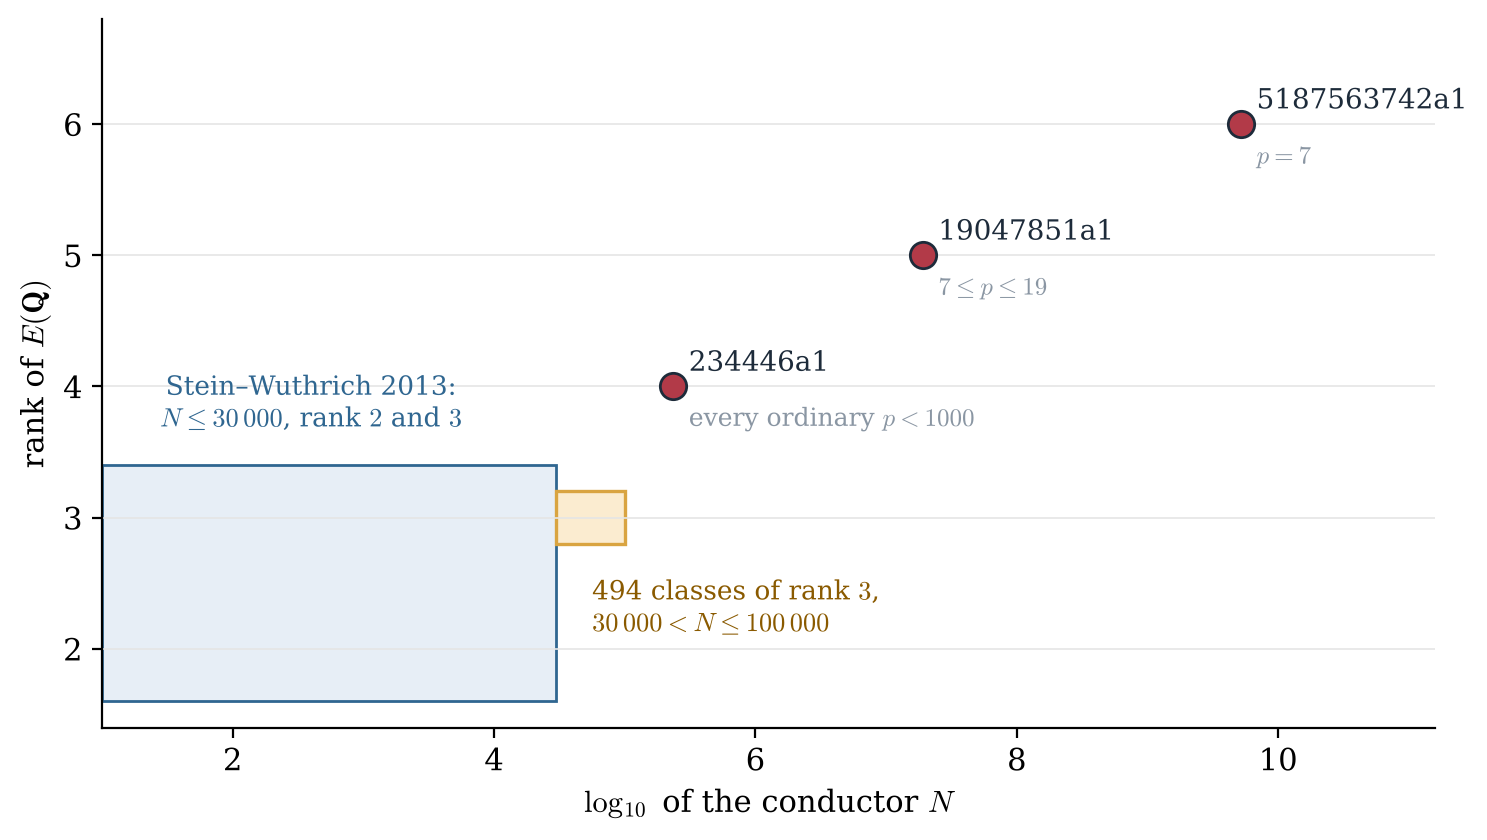
\includegraphics[width=0.9\textwidth]{figures/fig_landscape.png}
\caption{Ranks and conductors covered. The shaded rectangle is the range of Stein and Wuthrich; the small box is Theorem~\ref{thm:B}; the three dots are Theorems~\ref{thm:A}, \ref{thm:C}, \ref{thm:D}, with the primes treated.}\label{fig:landscape}
\end{figure}

\subsection{What the method does not reach}
The theorems are statements about one prime at a time. They do not show that $\Sha(E/\Q)$ is finite for any of these curves: the primes $2$ and $3$ for $E_5$ and $E_6$, the prime $3$ for $E_4$, the primes $2$, $3$ and the primes of bad or supersingular reduction for the curves of Theorem~\ref{thm:B}, and all primes above the bounds remain. Nor do they touch the complex side of \eqref{eq:bsd}. For $E_4$ the sign of the functional equation is $+1$ and the modular symbol $[0]^+$ vanishes, so $L(E_4,1)=L'(E_4,1)=0$; numerically $L(E_4,s)$ vanishes to order four at $s=1$, but no method is known that proves $L''(E_4,1)=0$, and so the first statement of \eqref{eq:bsd} is open for $E_4$, as it is for every curve of rank at least four. Section~\ref{sec:gap} describes what would be needed to pass from these $p$-adic statements to the conjecture itself.

\subsection{The argument and the plan}
The proof of each case has the same shape, drawn in Figure~\ref{fig:logic}. Sections~\ref{sec:symbols}--\ref{sec:iwasawa} recall the $p$-adic $L$-function, the $p$-adic height and the two theorems of Iwasawa theory on which everything rests, and prove the elementary facts about them that the argument uses: integrality of the modular symbols, the distribution relation, and a bound for the error of the Riemann sums that approximate $L_p(E,T)$. Section~\ref{sec:criterion} proves the criterion (Theorem~\ref{thm:criterion}) that turns one congruence between two explicit numbers into the conclusions above. Sections~\ref{sec:surj} and~\ref{sec:sat} give the two side conditions---surjectivity of $\rhobar$ and $p$-saturation of the points---in a form that can be checked by counting points on reductions. Sections~\ref{sec:rank4}--\ref{sec:rank56} prove Theorems~\ref{thm:A}--\ref{thm:D}; for $E_4$ at $p=5$ and for $E_5$ at $p=7$ the whole verification is carried out in the text from a handful of modular symbols. Section~\ref{sec:leading} compares the leading coefficients beyond their valuations, and Section~\ref{sec:gap} discusses the distance to the conjecture. The appendices contain the proofs of the auxiliary lemmas, the subgroups of $\GL_2(\F_p)$, the $p$-adic sigma function in closed form, and the tables.

Finite certificates of this kind---explicit data that reduce a theorem to arithmetic anyone can redo---accompany several recent computations on character sums, totients and modular forms \cite{BhaPV,BhaLehmer,BhaSen}.

\begin{figure}[t]
\centering
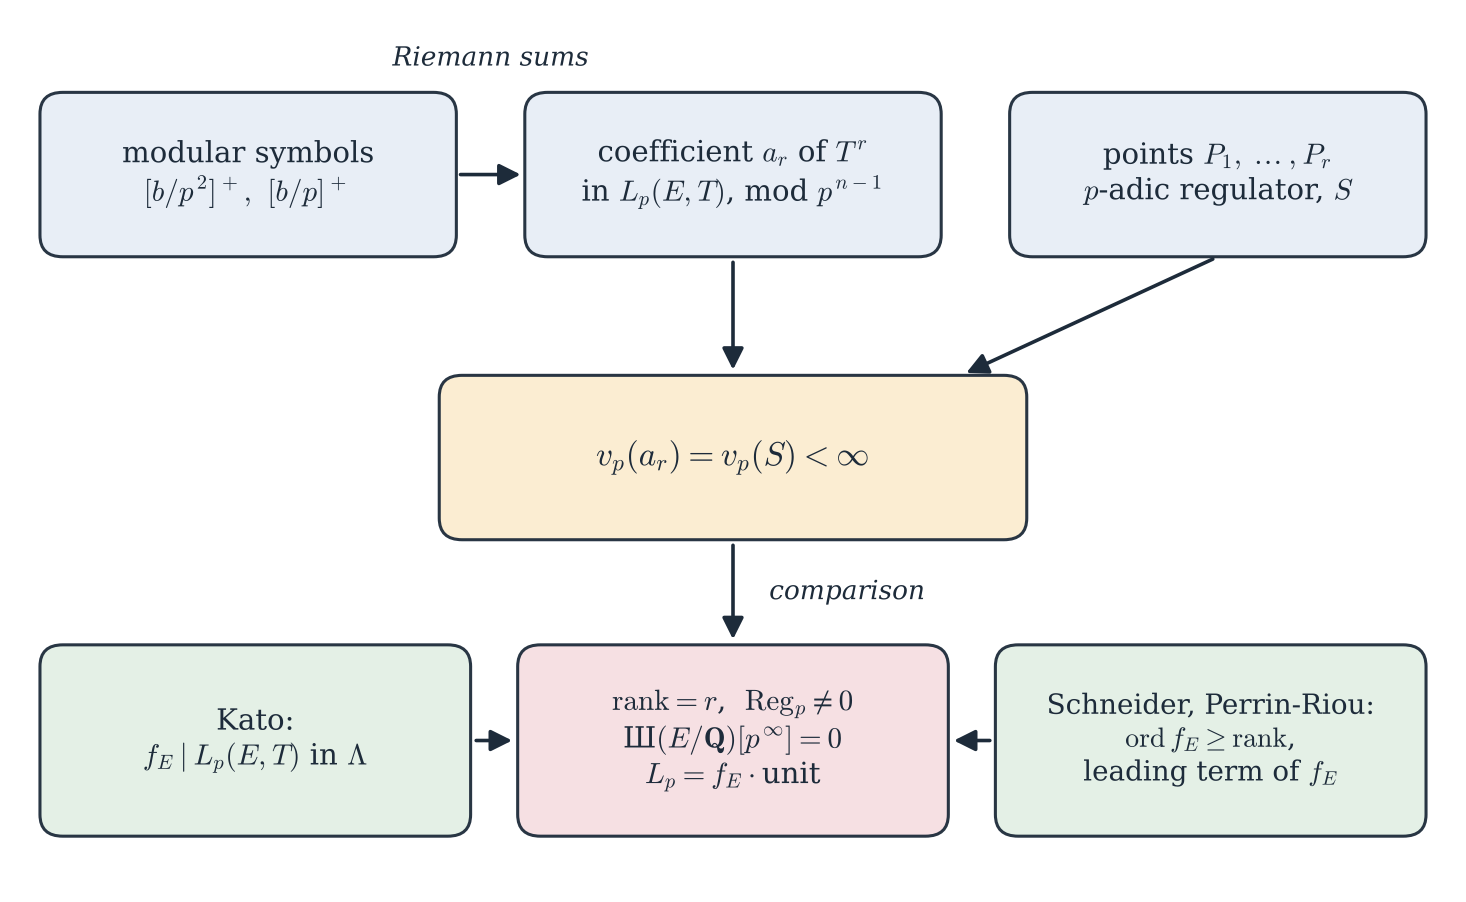
\includegraphics[width=0.92\textwidth]{figures/fig_logic.png}
\caption{The structure of the proof of Theorem~\ref{thm:criterion}. The top row is computed; the bottom corners are the two theorems of Iwasawa theory used.}\label{fig:logic}
\end{figure}

\subsection*{Notation}
Throughout, $p$ is an odd prime, $v_p$ the $p$-adic valuation on $\Qp$ with $v_p(0)=\infty$, $\log_p$ the Iwasawa logarithm, and $\Lambda=\Zp[[T]]$. For an elliptic curve $E/\Q$ we write $a_\ell$ for the trace of Frobenius at a good prime $\ell$, so that $\#\tilde E(\F_\ell)=\ell+1-a_\ell$, and $\rhobar\colon\Gal(\bar\Q/\Q)\to\GL_2(\F_p)$ for the action on $E[p]$. The prime $p$ is \emph{good ordinary} if $p\nmid N$ and $p\nmid a_p$; then $X^2-a_pX+p$ has exactly one root $\alpha\in\Zp^\times$.

\section{Modular symbols and the \texorpdfstring{$p$}{p}-adic \texorpdfstring{$L$}{L}-function}\label{sec:symbols}

\subsection{Modular symbols}
Let $f=\sum a_nq^n$ be the newform attached to $E$. For $r\in\Q$ put $\lambda(r)=2\pi i\int_r^{i\infty}f(\tau)\,d\tau$, the integral taken along a vertical line, and
\[
\lambda^+(r)=-\tfrac12\bigl(\lambda(r)+\lambda(-r)\bigr),\qquad [r]^+=\frac{\lambda^+(r)}{\Omega_E}.
\]
Since $f$ has real coefficients, $\lambda(-r)=\overline{\lambda(r)}$ and $\lambda^+(r)$ is real. The function $r\mapsto[r]^+$ is the \emph{plus modular symbol} of $E$; at $r=0$ it gives $[0]^+=L(E,1)/\Omega_E$.\footnote{With the orientation used here $\lambda(0)=2\pi i\int_0^{i\infty}f=-L(E,1)$, the integral $\int_0^{i\infty}f(\tau)\,d\tau$ being $iL(E,1)/(2\pi)$; the sign in the definition of $\lambda^+$ compensates. The proofs use only $p$-adic valuations, which a sign or a factor $2$ does not change. The congruences between $a_r$ and $S_p$ reported in \S\S\ref{sec:rank4}--\ref{sec:rank56} do depend on the normalisation, and they hold for the one fixed here: division by the N\'eron period $\Omega_E$, which is twice the least positive real period when $E(\R)$ has two components.} The following three properties are all that is used.

\begin{lemma}\label{lem:symbols}
Let $r\in\Q$.
\begin{enumerate}
\item[(a)] $[r+1]^+=[r]^+$ and $[-r]^+=[r]^+$.
\item[(b)] For every prime $\ell\nmid N$,
$\displaystyle a_\ell\,[r]^+=\sum_{b=0}^{\ell-1}\Bigl[\frac{r+b}{\ell}\Bigr]^+ +[\ell r]^+ .$
\item[(c)] Let $p$ be an odd prime with $p\nmid N$ and $E[p]$ irreducible as a Galois module. If the denominator of $r$ is prime to $N$, then $[r]^+\in\Z_{(p)}$.
\end{enumerate}
\end{lemma}

Parts (a) and (b) are proved in Appendix~\ref{app:hecke}. Part (c) rests on the theorem of Manin and Drinfeld \cite{Man72,Dri73} and on Edixhoven's theorem that the Manin constant of an optimal curve is an integer \cite{Edi91}; since the argument is short we give it here.

\begin{proof}[Proof of (c)]
We first show that every isogeny $\psi$ between $E$ and a curve $E'$ isogenous to it can be chosen of degree prime to $p$. Any isogeny factors as a multiplication map followed by an isogeny with cyclic kernel, so it is enough to consider cyclic kernels $C$. If $p$ divided $\#C$, then $C$ would contain a unique subgroup of order $p$; it would be stable under $\Gal(\bar\Q/\Q)$, because $C$ is, and it would be a line in $E[p]$ fixed by Galois, contradicting irreducibility. Hence $p\nmid\#C$.

Let $E_0$ be the optimal curve in the isogeny class of $E$, with modular parametrisation $\pi_0\colon X_0(N)\to E_0$ and Manin constant $c_0$, so that $c_0\,\pi_0^*\omega_{E_0}=2\pi i f(\tau)\,d\tau$ for the N\'eron differential $\omega_{E_0}$; by \cite{Edi91}, $c_0\in\Z$. Choose $\psi\colon E_0\to E$ of degree $d$ prime to $p$ and put $\pi=\psi\circ\pi_0$. N\'eron differentials pull back to integral multiples under isogenies, so $\psi^*\omega_E=m\,\omega_{E_0}$ and $\hat\psi^*\omega_{E_0}=m'\omega_E$ with $m,m'\in\Z$; since $\psi\circ\hat\psi$ is multiplication by $d$ we get $mm'=d$, hence $p\nmid m$. Thus $c\,\pi^*\omega_E=2\pi i f\,d\tau$ with $c=c_0/m\in\Z_{(p)}$.

Write $r=a/s$ in lowest terms with $\gcd(s,N)=1$. Since $\gcd(s,aN)=1$ there are integers $x,y$ with $xs-yaN=1$. The matrix $\left(\begin{smallmatrix} x & a\\ yN & s\end{smallmatrix}\right)$ then lies in $\Gamma_0(N)$, and it sends $0$ to $a/s=r$. So $r$ and $0$ are the same cusp of $X_0(N)$, and a path from $r$ to $0$ in the upper half-plane maps to a closed loop on $X_0(N)$. Therefore
\[
\lambda(r)-\lambda(0)=2\pi i\int_r^0 f(\tau)\,d\tau = c\int_{\pi(\text{loop})}\omega_E\in c\,\Lambda_E ,
\]
where $\Lambda_E$ is the period lattice of $\omega_E$. Next, $\lambda(0)=c\int_{\pi(0)}^{\pi(\infty)}\omega_E$ is an elliptic logarithm of the point $Q=\pi(\infty)-\pi(0)\in E$. The cusps $0$ and $\infty$ are rational points of $X_0(N)$, so $Q\in E(\Q)$, and $Q$ is a torsion point by the theorem of Manin and Drinfeld. Its order $t$ divides $\#E(\Q)_\tors$, which is prime to $p$ because $E(\Q)[p]$ is a Galois-stable subspace of the irreducible module $E[p]$ and is therefore $0$. Hence $\lambda(\pm r)\in (c/t)\Lambda_E$ and $\lambda^+(r)\in\frac{c}{2t}\Lambda_E\cap\R=\frac{c}{2t}\Z\,\Omega_0$, where $\Omega_0$ is the least positive real period. Finally $\Omega_E=c_\infty\Omega_0$ with $c_\infty\in\{1,2\}$ the number of connected components of $E(\R)$, so $[r]^+\in\frac{c}{2tc_\infty}\Z\subset\Z_{(p)}$.
\end{proof}

\subsection{How the symbols are evaluated}\label{ssec:manin}
The values $[r]^+$ are rational numbers, and they can be found exactly by a finite computation. The device is Manin's: a path from $\infty$ to a rational number is cut into unimodular pieces by the continued fraction of that number, and each piece is carried by an element of $\SL_2(\Z)$ to the path from $0$ to $\infty$.

Let $r=a/s$ with $s\ge1$ and $\gcd(a,s)=1$, and let $p_k/q_k$ for $0\le k\le m$ be the convergents of its continued fraction, with $p_m/q_m=a/s$, and $p_{-1}/q_{-1}=1/0$. They satisfy $p_kq_{k-1}-p_{k-1}q_k=(-1)^{k-1}$, so
\[
g_k=\begin{pmatrix}p_k&(-1)^{k-1}p_{k-1}\\ q_k&(-1)^{k-1}q_{k-1}\end{pmatrix}\in\SL_2(\Z),\qquad g_k\cdot0=\frac{p_{k-1}}{q_{k-1}},\quad g_k\cdot\infty=\frac{p_k}{q_k}.
\]
Write $\{\alpha,\beta\}$ for the path from $\alpha$ to $\beta$ in the upper half-plane together with the cusps. Then $\{\infty,r\}=\sum_{k=0}^{m}\{g_k0,g_k\infty\}$, and therefore
\begin{equation}\label{eq:manin}
\lambda(r)=-\sum_{k=0}^{m}\xi\bigl(q_k:(-1)^{k-1}q_{k-1}\bigr),\qquad \xi(c:d)=2\pi i\int_{g\cdot0}^{g\cdot\infty}f(\tau)\,d\tau ,
\end{equation}
where $g\in\SL_2(\Z)$ is any matrix with bottom row $(c,d)$. The integral in the definition of $\xi$ depends only on the coset $\Gamma_0(N)g$, because $f(\gamma\tau)\,d(\gamma\tau)=f(\tau)\,d\tau$ for $\gamma\in\Gamma_0(N)$, and that coset is determined by the point $(c:d)$ of $\mathbf P^1(\Z/N\Z)$. So $\xi$ is a function on the finite set $\mathbf P^1(\Z/N\Z)$, of cardinality $N\prod_{\ell\mid N}(1+\ell^{-1})$; its values are the \emph{Manin symbols} of $f$.

Two consequences matter here. First, the number of terms in \eqref{eq:manin} is the length of the continued fraction, which is $O(\log s)$; a symbol with denominator $p^n$ costs $O(n\log p)$ table look-ups once the Manin symbols are known. Second, the Manin symbols satisfy the relations $\xi(x)+\xi(xS)=0$ and $\xi(x)+\xi(xU)+\xi(xU^2)=0$, with $S=\left(\begin{smallmatrix}0&-1\\1&0\end{smallmatrix}\right)$ and $U=\left(\begin{smallmatrix}0&-1\\1&-1\end{smallmatrix}\right)$ (they come from the paths $\{0,\infty\}+\{\infty,0\}=0$ and $\{0,\infty\}+\{\infty,1\}+\{1,0\}=0$), and they are eigenvectors of the Hecke operators. Cremona's method \cite[Ch.~2]{Cre97} solves this finite system of linear equations over $\Q$ and isolates the eigenvector of $f$; the result, scaled by the period, gives the exact values of $[r]^+$. This is how the symbols for the curves of conductor below $250\,000$ were computed. For the two curves of rank five and six the space is too large, and Section~\ref{sec:rank56} uses a numerical method with a proven error bound instead.

\subsection{The measure}
Let $p\nmid N$ be good ordinary, with unit root $\alpha$. For $k\ge1$ and $a\in\Z$ prime to $p$ put
\begin{equation}\label{eq:mu}
\mu(a+p^k\Zp)=\frac{1}{\alpha^{k}}\Bigl[\frac{a}{p^k}\Bigr]^+-\frac{1}{\alpha^{k+1}}\Bigl[\frac{a}{p^{k-1}}\Bigr]^+ .
\end{equation}
By Lemma~\ref{lem:symbols}(a) the right side depends only on $a$ modulo $p^k$.

\begin{lemma}\label{lem:distribution}
The function $\mu$ is additive on the compact open subsets of $\Zp^\times$: for $k\ge1$ and $a$ prime to $p$,
$\sum_{b=0}^{p-1}\mu(a+bp^k+p^{k+1}\Zp)=\mu(a+p^k\Zp)$.
If $E[p]$ is irreducible, $\mu$ takes values in $\Zp$.
\end{lemma}

\begin{proof}
By Lemma~\ref{lem:symbols}(a), $[(a+bp^k)/p^k]^+=[a/p^k]^+$, so
\[
\sum_{b}\mu(a+bp^k+p^{k+1}\Zp)=\alpha^{-k-1}\sum_{b}\Bigl[\frac{a/p^k+b}{p}\Bigr]^+-\alpha^{-k-2}\,p\,\Bigl[\frac{a}{p^k}\Bigr]^+ .
\]
Lemma~\ref{lem:symbols}(b) with $\ell=p$ and $r=a/p^k$ turns the first sum into $a_p[a/p^k]^+-[a/p^{k-1}]^+$. Write $\beta=p/\alpha$, the other root, so that $a_p-p/\alpha=\alpha$. The total becomes $\alpha^{-k-1}\bigl(\alpha[a/p^k]^+-[a/p^{k-1}]^+\bigr)=\mu(a+p^k\Zp)$. Integrality follows from Lemma~\ref{lem:symbols}(c), as $\alpha\in\Zp^\times$ and the denominators $p^k$ are prime to $N$.
\end{proof}

A finitely additive $\Zp$-valued function on the compact open sets of $\Zp^\times$ is a measure, and continuous functions $\Zp^\times\to\Zp$ can be integrated against it as limits of Riemann sums.

\subsection{The \texorpdfstring{$p$}{p}-adic \texorpdfstring{$L$}{L}-function}
Every $x\in\Zp^\times$ factors uniquely as $x=\omega(x)\langle x\rangle$ with $\omega(x)^{p-1}=1$ and $\langle x\rangle\in1+p\Zp$. The logarithm maps $1+p\Zp$ isomorphically onto $p\Zp$, and $v_p(\log_p(1+p))=1$, so
\[
\ell(x)=\frac{\log_p\langle x\rangle}{\log_p(1+p)}\in\Zp
\]
and $\langle x\rangle=(1+p)^{\ell(x)}$. Following \cite{MTT86} and \cite[\S3]{SW13} we define
\begin{equation}\label{eq:Lp}
L_p(E,T)=\int_{\Zp^\times}(1+T)^{\ell(x)}\,d\mu(x)=\sum_{k\ge0}a_kT^k,\qquad a_k=\int_{\Zp^\times}\binom{\ell(x)}{k}d\mu(x).
\end{equation}
Since $s\mapsto\binom{s}{k}$ maps $\Zp$ to $\Zp$ continuously and $\mu$ is $\Zp$-valued, every $a_k$ lies in $\Zp$: \emph{$L_p(E,T)\in\Lambda$ whenever $E[p]$ is irreducible}. At $T=0$ the integral is the total mass, $a_0=(1-\alpha^{-1})^2[0]^+$ (from \eqref{eq:mu} with $k=1$ and Lemma~\ref{lem:symbols}(b)), which is the interpolation property at the trivial character.

The coefficients are computed by Riemann sums. As $a$ runs through $1,\dots,p-1$ and $j$ through $0,\dots,p^{n-1}-1$, the numbers $\omega(a)(1+p)^j$ run once through a set of representatives of $(\Z/p^n\Z)^\times$, and $\ell(\omega(a)(1+p)^j)=j$. Put
\begin{equation}\label{eq:riemann}
L_{p,n}(T)=\sum_{a=1}^{p-1}\sum_{j=0}^{p^{n-1}-1}\mu\bigl(\omega(a)(1+p)^j+p^n\Zp\bigr)\,(1+T)^j=\sum_k a_{n,k}T^k .
\end{equation}

\begin{proposition}\label{prop:precision}
Suppose $E[p]$ is irreducible, $n\ge2$ and $1\le k$. Then
\[
a_k\equiv a_{n,k}\pmod{p^{\,n-1-e_k}},\qquad e_k=\max_{1\le i\le k}v_p(i).
\]
In particular $a_k\equiv a_{n,k}\pmod{p^{n-1}}$ for $k<p$.
\end{proposition}

The proof is in Appendix~\ref{app:precision}. The same bound, in a slightly different form, is \cite[Prop.~3.5]{SW13}.\footnote{Stein and Wuthrich compare consecutive Riemann sums through the divisibility of $L_{p,n+1}-L_{p,n}$ by $(1+T)^{p^{n-1}}-1$; the proof in Appendix~\ref{app:precision} instead estimates the oscillation of $(1+T)^{\ell(x)}$ on each residue class, which gives the bound in one step.}

For $n=2$ the proposition gives every coefficient $a_k$ with $k<p$ modulo $p$ from finitely many rational numbers. Indeed $\omega(a)\equiv a^p\pmod{p^2}$, $\alpha\equiv a_p\pmod p$, and $[b/p]^+=[a/p]^+$ when $b\equiv a\pmod p$, so, writing $b_{a,j}$ for the residue of $a^p(1+p)^j$ modulo $p^2$,
\begin{equation}\label{eq:closed}
a_k\equiv\sum_{j=k}^{p-1}\binom{j}{k}\sum_{a=1}^{p-1}\Bigl(a_p^{-2}\Bigl[\frac{b_{a,j}}{p^2}\Bigr]^+-a_p^{-3}\Bigl[\frac{a}{p}\Bigr]^+\Bigr)\pmod p\qquad(1\le k<p).
\end{equation}
At the irregular pairs the second level is not enough, and the same computation is carried out at level $n\ge3$. The symmetry $[-r]^+=[r]^+$ then halves the work.

\begin{proposition}\label{prop:leveln}
Let $n\ge2$, $1\le k<p$, and let $b_{a,j}$ be the residue of $a^{p^{n-1}}(1+p)^j$ modulo $p^n$. Then
\[
a_k\equiv2\sum_{j=k}^{p^{n-1}-1}\binom{j}{k}\sum_{a=1}^{(p-1)/2}\Bigl(\alpha^{-n}\Bigl[\frac{b_{a,j}}{p^n}\Bigr]^+-\alpha^{-n-1}\Bigl[\frac{b_{a,j}}{p^{n-1}}\Bigr]^+\Bigr)\pmod{p^{n-1}} .
\]
\end{proposition}

\begin{proof}
The Teichm\"uller character satisfies $\omega(a)\equiv a^{p^{n-1}}\pmod{p^n}$: indeed $a^{p^{n-1}}=\omega(a)^{p^{n-1}}\langle a\rangle^{p^{n-1}}$, and $\omega(a)^{p^{n-1}}=\omega(a)$ because $p^{n-1}\equiv1\pmod{p-1}$, while $\langle a\rangle^{p^{n-1}}\in1+p^n\Zp$. So $b_{a,j}$ represents $\omega(a)(1+p)^j$ modulo $p^n$, and $\binom{j}{k}=0$ for $j<k$. Since $\omega(p-a)=\omega(-1)\omega(a)=-\omega(a)$, we have $b_{p-a,j}\equiv-b_{a,j}$, and \eqref{eq:mu} together with Lemma~\ref{lem:symbols}(a) gives $\mu(-b+p^n\Zp)=\mu(b+p^n\Zp)$. The terms for $a$ and $p-a$ in \eqref{eq:riemann} are therefore equal, and Proposition~\ref{prop:precision} finishes the proof.
\end{proof}

For $n=2$ this is \eqref{eq:closed}, with $\alpha\equiv a_p\pmod p$. For $n=3$ and $n=4$ it requires $\alpha$ modulo $p^2$ and $p^3$, which Hensel's lemma gives from $\alpha\equiv a_p\pmod p$, and the symbols $[b/p^n]^+$ for about $\frac12p^{n}$ residues $b$. At $p=89$ and $n=4$ this is $3.1\cdot10^7$ symbols, the largest computation in the paper.

The function $L_p(E,T)$ defined in \eqref{eq:Lp} is the $p$-adic $L$-function of Mazur, Tate and Teitelbaum: it interpolates the twisted values $L(E,\chi,1)$. This is not used in the proofs, but it explains why Kato's theorem below, which concerns their function, applies to ours.

\begin{proposition}\label{prop:interp}
Let $\chi$ be a primitive even Dirichlet character of conductor $p^n$, $n\ge1$, and $G(\chi)=\sum_{a\bmod p^n}\chi(a)e^{2\pi ia/p^n}$. Then
\[
\int_{\Zp^\times}\chi\,d\mu=\frac{G(\chi)}{\alpha^{n}}\cdot\frac{L(E,\bar\chi,1)}{\Omega_E}.
\]
In particular, if $n\ge2$ and $\chi$ is a character of order $p^{n-1}$ trivial on the roots of unity in $\Zp^\times$, then $\zeta=\chi(1+p)$ is a primitive $p^{n-1}$-th root of unity and $L_p(E,\zeta-1)$ is this value.
\end{proposition}

\begin{proof}
Put $m=p^n$. The second term of \eqref{eq:mu} contributes $\alpha^{-n-1}\sum_{c\bmod p^{n-1}}[c/p^{n-1}]^+\sum_{a\equiv c}\chi(a)$, and the inner sums vanish because $\chi$ is primitive of conductor $m$. So $\int\chi\,d\mu=\alpha^{-n}\sum_a\chi(a)[a/m]^+$. Next, $\lambda(a/m)=2\pi i\int_0^{i\infty}f(\tau+a/m)\,d\tau$, and the orthogonality of additive characters gives
\[
\sum_{a\bmod m}\chi(a)f\Bigl(\tau+\frac am\Bigr)=\sum_{n'\ge1}a_{n'}q^{n'}\sum_a\chi(a)e^{2\pi ian'/m}=G(\chi)\sum_{n'}\bar\chi(n')a_{n'}q^{n'},
\]
the last step because $\sum_a\chi(a)e^{2\pi ian'/m}=\bar\chi(n')G(\chi)$ for primitive $\chi$. Integrating, $\sum_a\chi(a)\lambda(a/m)=-G(\chi)L(E,\bar\chi,1)$, with the normalisation of the footnote above. As $\chi$ is even, $\sum_a\chi(a)\lambda(-a/m)=\sum_a\chi(a)\lambda(a/m)$, so $\sum_a\chi(a)\lambda^+(a/m)=G(\chi)L(E,\bar\chi,1)$. Dividing by $\Omega_E$ proves the formula. For the last statement, such a character is even, it has conductor $p^n$, and $\chi(x)=\chi(\langle x\rangle)=\zeta^{\ell(x)}$, and $\int\zeta^{\ell(x)}d\mu=L_p(E,\zeta-1)$ by \eqref{eq:Lp}.
\end{proof}

The two formulas \eqref{eq:closed} and Proposition~\ref{prop:leveln} are what the proofs of Theorems~\ref{thm:A}--\ref{thm:D} evaluate.

\section{\texorpdfstring{$p$}{p}-adic heights}\label{sec:heights}

Let $p$ be good ordinary for $E$. The cyclotomic $p$-adic height was defined by Schneider \cite{Sch82} and Perrin-Riou; we use the explicit description of Mazur and Tate \cite{MT91} in the normalisation of \cite[\S4]{SW13}, and compute it by the algorithm of Mazur, Stein and Tate \cite{MST06}. Let $t=-x/y$ be the parameter at the origin of a minimal model, $\omega_E=dx/(2y+a_1x+a_3)$ and $b_2=a_1^2+4a_2$. The \emph{canonical $p$-adic sigma function} $\sigma_p(t)\in t+t^2\Zp[[t]]$ is the unique function of the form $\sigma_p=t+\cdots$, odd for the inverse map of the formal group, satisfying
\[
x+c=-\frac{d}{\omega_E}\Bigl(\frac{1}{\sigma_p}\frac{d\sigma_p}{\omega_E}\Bigr),\qquad c=\frac{b_2-e_2}{12},
\]
where $e_2=E_2(E,\omega_E)$ is the value of Katz's $p$-adic Eisenstein series of weight two \cite{Kat76}; Mazur and Tate proved that $\sigma_p$ has coefficients in $\Zp$ \cite{MT91}. Appendix~\ref{app:sigma} gives $\sigma_p$ in closed form, characterises $c$ through Frobenius, and works the example of $E_4$ at $5$. If $P\in E(\Q)$ reduces to the identity modulo $p$ and to the identity component of the N\'eron model at every prime, and $e(P)$ is the positive square root of the denominator of $x(P)$, put
\[
\hat h_p(P)=2\log_p\frac{e(P)}{\sigma_p(P)} ,
\]
and extend to all of $E(\Q)$ by $\hat h_p(mP)=m^2\hat h_p(P)$. This is a quadratic form, and
\[
\langle P,Q\rangle_p=\tfrac12\bigl(\hat h_p(P+Q)-\hat h_p(P)-\hat h_p(Q)\bigr)
\]
is a symmetric bilinear form on $E(\Q)/E(\Q)_\tors$ with values in $\Qp$. For points $P_1,\dots,P_r$ put
\[
\Reg_p(P_1,\dots,P_r)=\det\bigl(\langle P_i,P_j\rangle_p\bigr),\qquad\Reg_\gamma=\frac{\Reg_p}{\log_p(1+p)^r},
\]
and write $\Reg_p(E/\Q)$, $\Reg_\gamma(E/\Q)$ for the values on a basis of $E(\Q)/E(\Q)_\tors$; they are well defined up to sign. The division by $\log_p(1+p)^r$ matches the choice of the generator $1+p$ of $1+p\Zp$ that identifies the Iwasawa algebra with $\Lambda$ \cite[\S4.4]{SW13}.

\begin{lemma}\label{lem:index}
If $P_1,\dots,P_r$ are independent and generate a subgroup of index $n$ in $E(\Q)/E(\Q)_\tors$, a free group of rank $r$, then $\Reg_p(P_1,\dots,P_r)=n^2\,\Reg_p(E/\Q)$.
\end{lemma}

\begin{proof}
If $(P_i)=A\,(Q_j)$ with $(Q_j)$ a basis and $A$ an integral matrix, then $|\det A|=n$ and the Gram matrices satisfy $G_P=AG_QA^{\mathsf T}$.
\end{proof}

The size of the regulator is controlled by the reduction of $E$ at $p$ and at the bad primes, and the following lemma explains the valuations that appear in the examples below.

\begin{lemma}\label{lem:heightval}
Let $m=\operatorname{lcm}\bigl(\#\tilde E(\F_p),c_v:v\mid N\bigr)$ and $k=v_p(m)$. Then $\langle P,Q\rangle_p\in p^{1-2k}\Zp$ for all $P,Q\in E(\Q)$, and $v_p(\Reg_p(P_1,\dots,P_r))\ge r(1-2k)$. In particular, if $p$ is not anomalous and divides no Tamagawa number, then $\Reg_\gamma(P_1,\dots,P_r)\in\Zp$.
\end{lemma}

\begin{proof}
Let $R=mP$, which reduces to the identity modulo $p$ and to the identity component at every bad prime. Write $x(R)=a/e^2$ and $y(R)=b/e^3$ in lowest terms, with $e=e(R)$. If $v_p(x(R))=-2j$ with $j\ge1$, then $v_p(e)=j$ and $p\nmid ab$, and $t(R)=-x/y=-ae/b$ has valuation $j$. So
\[
\frac{e(R)}{\sigma_p(R)}=\frac{e}{t(R)}\cdot\frac{t(R)}{\sigma_p(R)}=-\frac ba\cdot\Bigl(\frac{\sigma_p(t)}{t}\Bigr)^{-1}\Big|_{t=t(R)},
\]
and both factors are units of $\Zp$: the first because $p\nmid ab$, the second because $\sigma_p(t)/t\in1+t\Zp[[t]]$ and $t(R)\in p\Zp$. For any $u\in\Zp^\times$ we have $u^{p-1}\in1+p\Zp$, so $\log_pu=\tfrac1{p-1}\log_p(u^{p-1})\in p\Zp$. Hence $\hat h_p(R)\in p\Zp$, and $\hat h_p(P)=m^{-2}\hat h_p(R)\in p^{1-2k}\Zp$. The pairing is half a sum of three such values, and $p$ is odd. The bound on the determinant follows by expanding it, and the last statement from $k=0$ and $v_p(\log_p(1+p))=1$.
\end{proof}

So when $p$ is not anomalous and divides no Tamagawa number, the factors $(1-\alpha^{-1})^2$ and $\prod c_v$ are units, and the pair $(E,p)$ is irregular exactly when $p^{r+1}$ divides $\Reg_p(E/\Q)$, that is, when the matrix $p^{-1}(\langle P_i,P_j\rangle_p)$ is singular modulo $p$. If this matrix behaved like a random symmetric matrix over $\F_p$, it would be singular with probability close to $1/p$. This is the heuristic behind \S\ref{sec:rank3}, and Figure~\ref{fig:irregular} bears it out. When $p$ is anomalous, $k\ge1$, and the entries may have negative valuation, as they do for $E_4$ at $5$ below.

\emph{Schneider's conjecture} asserts that $\Reg_p(E/\Q)\neq0$ for every $p$. For curves of rank one with complex multiplication it is a theorem of Bertrand, proved by transcendence methods; beyond that case no general result is known.\footnote{See \cite{SW13} for references. For a given curve and prime the nonvanishing is decided by computing the pairing to sufficient precision, which is how it is established for the curves of this paper.}

\subsection{Computing the pairing}\label{ssec:heightcomp}
Three steps turn the definition into numbers \cite{MST06}. The value $e_2$ is read off from the eigenline of Frobenius with unit eigenvalue in the de Rham cohomology $H^1_{\mathrm{dR}}(E/\Qp)$, written in the basis $\omega,\ x\omega$; the matrix of Frobenius on this two-dimensional space is computed by Kedlaya's algorithm, and that eigenline is found by iterating it. The function $\sigma_p$ is then given by the closed formula of Proposition~\ref{prop:sigmaclosed}, to any prescribed $t$-adic and $p$-adic precision. Finally, for a point $P$ one takes an integer $m$ such that $mP$ reduces to the identity modulo $p$ and to the identity component at the primes of bad reduction; $m=\operatorname{lcm}(\#\tilde E(\F_p),c_v)$ will do, since the component group at $v$ has order $c_v$. Then $\hat h_p(P)=m^{-2}\hat h_p(mP)$, and $mP$ lies in the domain of convergence of $\sigma_p$ because $t(mP)\in p\Zp$.

For $E_4$ and $p=5$ one may take $m=10$, as $\#\tilde E_4(\F_5)=10$ and $c_2=2$. The resulting Gram matrix has entries of valuation $-1$, $0$ and $1$; for instance
\[
\langle P_1,P_1\rangle_5=2\cdot5^{-1}+1+5+2\cdot5^2+O(5^3),\qquad \langle P_1,P_2\rangle_5=4+4\cdot5+4\cdot5^2+O(5^3).
\]
Clearing the denominator, the integer matrix
\[
N=\begin{pmatrix}
51532&28745&18034&44467\\
28745&25950&46565&66895\\
18034&46565&64483&37404\\
44467&66895&37404&20752
\end{pmatrix}
\]
satisfies $N\equiv5\bigl(\langle P_i,P_j\rangle_5\bigr)_{i,j}\pmod{5^7}$. Its determinant is $-1\,409\,401\,157\,357\,234\,375$, which is $2\cdot5^6$ modulo $5^7$, so
\[
\Reg_5(P_1,\dots,P_4)=5^{-4}\det N+O(5^3)=2\cdot5^2+O(5^3).
\]
Since every entry has valuation at least $-1$, the determinant could have valuation as low as $-4$; it has valuation $2$, so six powers of $5$ cancel in its expansion. In Section~\ref{ssec:p5} the valuation $2$ of $\Reg_5$, the valuation $-4$ of $\log_5(6)^{-4}$ and the valuation $2$ of the anomalous factor $(1-\alpha^{-1})^2$ add up to $0$, and this is what makes $v_5(S_5)=0$.

\section{Iwasawa theory}\label{sec:iwasawa}

\begin{figure}[t]
\centering
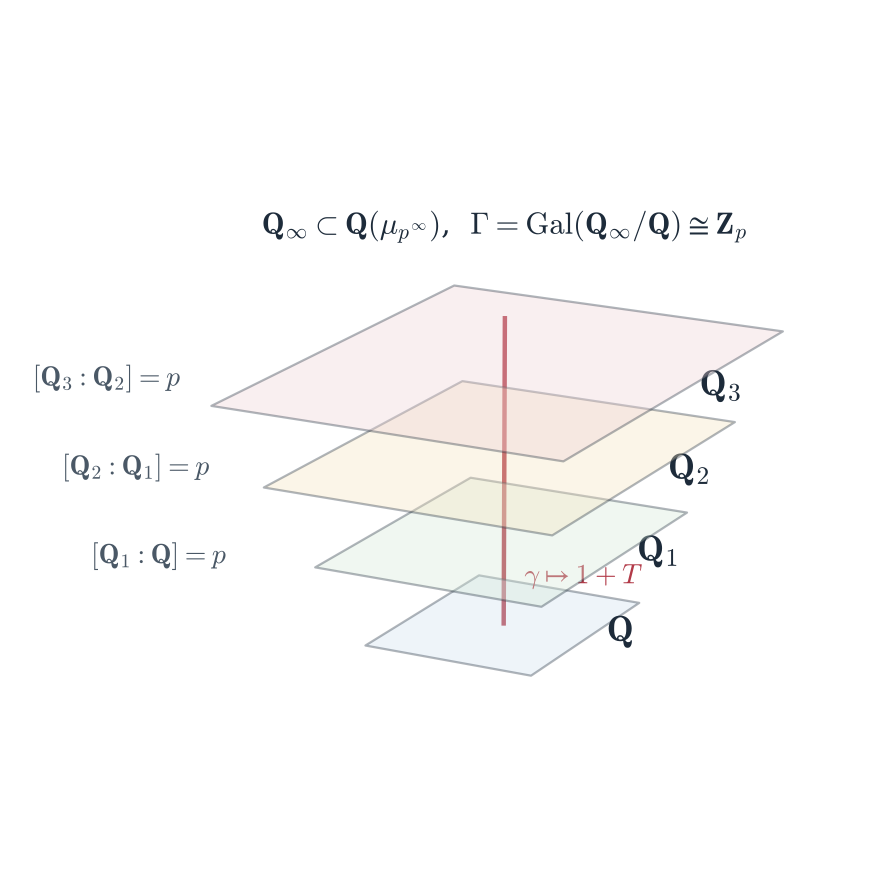
\includegraphics[width=0.62\textwidth]{figures/fig_tower.png}
\caption{The cyclotomic $\Z_p$-extension. The Selmer groups of $E$ over the layers $\Q_n$ are assembled into a module over $\Lambda=\Zp[[\Gamma]]$, with a generator $\gamma$ of $\Gamma$ acting as $1+T$.}\label{fig:tower}
\end{figure}

Let $\Q_\infty$ be the unique $\Z_p$-extension of $\Q$ contained in $\Q(\mu_{p^\infty})$, with layers $\Q_n$ of degree $p^n$ and Galois group $\Gamma$ (Figure~\ref{fig:tower}). The element $\gamma\in\Gamma$ acting on $\mu_{p^\infty}$ through the cyclotomic character by $1+p$ is a topological generator, and $\gamma\mapsto1+T$ identifies $\Zp[[\Gamma]]$ with $\Lambda$. Let
\[
\Sel_{p^\infty}(E/\Q_\infty)=\varinjlim_n\Sel_{p^\infty}(E/\Q_n),\qquad X(E/\Q_\infty)=\mathrm{Hom}\bigl(\Sel_{p^\infty}(E/\Q_\infty),\Q_p/\Z_p\bigr),
\]
a finitely generated $\Lambda$-module. When $p$ is good ordinary, Kato proved that $X(E/\Q_\infty)$ is $\Lambda$-torsion \cite[Thm.~17.4]{Kat04}, using Rohrlich's nonvanishing theorem \cite{Roh84}; let $f_E(T)\in\Lambda$ be a generator of its characteristic ideal, well defined up to a unit of $\Lambda$.

\begin{theorem}[Kato]\label{thm:kato}
Let $p\ge5$ be good ordinary for $E$ and suppose that $\rhobar$ is surjective. Then $f_E(T)$ divides $L_p(E,T)$ in $\Lambda$.
\end{theorem}

This is \cite[Thm.~17.4]{Kat04}, in the form stated in \cite[Thm.~7.3]{SW13}.\footnote{Kato's theorem is stated for the $p$-adic representation $\rho_{E,p}$ on the Tate module. For $p\ge5$ surjectivity of $\rhobar$ implies surjectivity of $\rho_{E,p}$: a closed subgroup of $\GL_2(\Zp)$ whose reduction is $\GL_2(\F_p)$ contains $\SL_2(\Zp)$ \cite[IV-23, Lemma~3]{Ser68}, and the determinant is the cyclotomic character, which is onto $\Zp^\times$.} Under the hypotheses of \cite{SU14} the divisibility is an equality, but this is not used.

\begin{theorem}[Schneider, Perrin-Riou]\label{thm:schneider}
Let $p$ be good ordinary for $E$ and $r=\rk E(\Q)$. Then $\ord_{T=0}f_E(T)\ge r$, with equality if and only if $\Reg_p(E/\Q)\neq0$ and $\Sha(E/\Q)[p^\infty]$ is finite. If equality holds, the coefficient $f_r$ of $T^r$ in $f_E$ satisfies
\[
v_p(f_r)=v_p\Bigl(\bigl(1-\alpha^{-1}\bigr)^2\cdot\frac{\prod_vc_v\cdot\#\Sha(E/\Q)[p^\infty]\cdot\Reg_\gamma(E/\Q)}{\#E(\Q)[p^\infty]^2}\Bigr).
\]
\end{theorem}

This is due to Schneider \cite{Sch85} and Perrin-Riou \cite{PR93}; see \cite[Thm.~6.1]{SW13}.\footnote{The inequality comes from Mazur's control theorem \cite{Maz72}: the $\Gamma$-coinvariants of $X(E/\Q_\infty)$ have $\Zp$-rank at least the corank of $\Sel_{p^\infty}(E/\Q)$, which is at least $r$. The factor $(1-\alpha^{-1})^2$ has valuation $2v_p(\#\tilde E(\F_p))$, so it is a unit unless $p$ is anomalous, $a_p\equiv1\pmod p$.}

\subsection{Where the inequality comes from}
The inequality in Theorem~\ref{thm:schneider} has a short proof from the structure of $\Lambda$-modules, and it shows where each factor of the leading term comes from.

For a number field $F$ the Selmer group $\Sel_{p^\infty}(E/F)\subset H^1(F,E[p^\infty])$ consists of the classes whose restriction to every completion lies in the image of the local Kummer map, and it sits in the exact sequence
\[
0\to E(F)\otimes\Q_p/\Z_p\to\Sel_{p^\infty}(E/F)\to\Sha(E/F)[p^\infty]\to0 .
\]
Hence its $\Zp$-corank $s_F$ satisfies $s_F\ge\rk E(F)$, with equality if and only if $\Sha(E/F)[p^\infty]$ is finite. Mazur's control theorem \cite{Maz72} (see also \cite{Gre99}) states that for $p$ good ordinary the restriction map
\[
\Sel_{p^\infty}(E/\Q)\longrightarrow\Sel_{p^\infty}(E/\Q_\infty)^{\Gamma}
\]
has finite kernel and cokernel. Dualising, $X(E/\Q_\infty)_\Gamma=X/TX$ has $\Zp$-rank $s_\Q\ge r$.

On the other side, by the structure theorem there is a homomorphism $X\to\bigoplus_i\Lambda/(g_i)$ with finite kernel and cokernel, where $g_i\in\Lambda$ and $f_E=\prod_ig_i$ up to a unit. Finite modules do not change $\Zp$-ranks of $T$-coinvariants, and $\Lambda/(g_i,T)=\Zp/(g_i(0))$ has rank one if $T\mid g_i$ and rank zero otherwise. Therefore
\[
r\le s_\Q=\rk_{\Zp}X/TX=\#\{i:\ T\mid g_i\}\le\ord_Tf_E .
\]
Equality throughout requires two things: $s_\Q=r$, that is, $\Sha(E/\Q)[p^\infty]$ finite; and that $T$ divide each $g_i$ at most once, so that $T$ acts semisimply on the $T$-primary part of $X$. Schneider showed that the second condition is governed by the $p$-adic height: when $\Sha(E/\Q)[p^\infty]$ is finite, the map from the $\Gamma$-invariants to the $\Gamma$-coinvariants of the Selmer group is given on $E(\Q)\otimes\Zp$ by the height pairing, so semisimplicity is equivalent to $\Reg_p(E/\Q)\ne0$ \cite{Sch85}. When both conditions hold, the leading coefficient $f_r$ is computed by following orders of finite groups through the control theorem. The cokernel of restriction contributes the Tamagawa numbers at the primes of bad reduction and the factor $\#\tilde E(\F_p)[p^\infty]^2$ at $p$, which for an ordinary prime equals the $p$-part of $(1-\alpha^{-1})^2$ up to a unit \cite{Gre99}; the finite group $\Sha(E/\Q)[p^\infty]$ contributes its order, and the height pairing contributes $\Reg_\gamma$.

\section{The criterion}\label{sec:criterion}

For independent points $P_1,\dots,P_r\in E(\Q)$ and a good ordinary prime $p$ put
\begin{equation}\label{eq:S}
S_p(P_1,\dots,P_r)=\bigl(1-\alpha^{-1}\bigr)^2\cdot\frac{\prod_vc_v\cdot\Reg_\gamma(P_1,\dots,P_r)}{\#E(\Q)_\tors^2}\in\Qp .
\end{equation}
The points are \emph{$p$-saturated} if no point $Q\in E(\Q)$ satisfies $pQ\in\sum\Z P_i+E(\Q)_\tors$ unless $Q\in\sum\Z P_i+E(\Q)_\tors$.

\begin{theorem}\label{thm:criterion}
Let $E/\Q$ be an elliptic curve and $p\ge5$ a good ordinary prime with $\rhobar$ surjective. Let $P_1,\dots,P_r\in E(\Q)$ be independent and $p$-saturated, and let $a_r$ be the coefficient of $T^r$ in $L_p(E,T)$. If
\begin{equation}\label{eq:test}
v_p(a_r)=v_p\bigl(S_p(P_1,\dots,P_r)\bigr)<\infty,
\end{equation}
then:
\begin{enumerate}
\item[(i)] $\rk E(\Q)=r$, and $P_1,\dots,P_r$ generate a subgroup of $E(\Q)/E(\Q)_\tors$ of index prime to $p$;
\item[(ii)] $\Sha(E/\Q)[p^\infty]=0$;
\item[(iii)] $\Reg_p(E/\Q)\ne0$ and $\ord_{T=0}L_p(E,T)=r$;
\item[(iv)] $L_p(E,T)=f_E(T)\,u(T)$ with $u\in\Lambda^\times$; that is, the main conjecture of Iwasawa theory holds for $(E,p)$.
\end{enumerate}
\end{theorem}

\begin{proof}
Surjectivity of $\rhobar$ gives three facts used repeatedly: $E[p]$ is irreducible, so $L_p(E,T)\in\Lambda$ by \S\ref{sec:symbols}; $E(\Q)[p]=0$, so $\#E(\Q)[p^\infty]=1$ and $\#E(\Q)_\tors$ is prime to $p$; and Theorem~\ref{thm:kato} applies. Write $L_p=f_E\,d$ with $d\in\Lambda$, and let $\rho=\rk E(\Q)\ge r$, the inequality because the $P_i$ are independent.

By Theorem~\ref{thm:schneider}, $\ord_Tf_E\ge\rho\ge r$, so the coefficients of $T^0,\dots,T^{r-1}$ of $L_p=f_Ed$ vanish and the coefficient of $T^r$ is
\[
a_r=f_r\,d(0),
\]
where $f_r$ is the coefficient of $T^r$ in $f_E$ (zero if $\ord_Tf_E>r$). By \eqref{eq:test}, $a_r\neq0$. Hence $f_r\ne0$, so $\ord_Tf_E=r$; together with $\ord_Tf_E\ge\rho\ge r$ this gives $\rho=r$ and, by the equality case of Theorem~\ref{thm:schneider}, $\Reg_p(E/\Q)\ne0$ and $\Sha(E/\Q)[p^\infty]$ finite. Also $d(0)\ne0$ and $\ord_TL_p=r$. This proves (iii) and the first half of (i).

Since $\rho=r$, the points $P_i$ generate a subgroup of finite index $n$ in $E(\Q)/E(\Q)_\tors$. Suppose $p\mid n$. The quotient then has an element of order $p$, represented by some $Q\notin\sum\Z P_i+E(\Q)_\tors$ with $pQ\in\sum\Z P_i+E(\Q)_\tors$, contradicting $p$-saturation. So $p\nmid n$, completing (i), and by Lemma~\ref{lem:index}, $v_p(S_p(P_1,\dots,P_r))=v_p(S_p(E))$, where $S_p(E)$ is \eqref{eq:S} evaluated on a basis.

Theorem~\ref{thm:schneider} now gives $v_p(f_r)=v_p(S_p(E))+v_p\#\Sha(E/\Q)[p^\infty]$. Since $d(0)\in\Zp$,
\[
v_p(S_p(E))+v_p\#\Sha(E/\Q)[p^\infty]=v_p(f_r)=v_p(a_r)-v_p(d(0))\le v_p(a_r)=v_p(S_p(E)),
\]
so $\#\Sha(E/\Q)[p^\infty]=1$ and $v_p(d(0))=0$. This is (ii), and $d(0)\in\Zp^\times$ means $d\in\Lambda^\times$, which is (iv).
\end{proof}

\begin{remark}\label{rem:low}
The proof does not use the coefficients $a_0,\dots,a_{r-1}$: their vanishing is a consequence of Theorems~\ref{thm:kato} and~\ref{thm:schneider}. When they are computed, their vanishing modulo the available power of $p$ is a check on the computation, and it held in every case treated below. Only $a_r$ modulo $p^{v_p(S)+1}$ is needed, and Proposition~\ref{prop:precision} with $n=v_p(S)+2$ supplies it when $r<p$. A pair with $v_p(S)>0$ is called \emph{irregular}; for those a deeper Riemann sum is required.
\end{remark}

\begin{remark}\label{rem:integral}
The quantity $S_p(E)$ is a product of factors that need not be integral individually, but the product is constrained. Suppose $\ord_Tf_E=\rk E(\Q)$. Since $f_E\in\Lambda$, its leading coefficient lies in $\Zp$, and Theorem~\ref{thm:schneider} gives
\[
v_p\bigl(S_p(E)\bigr)+v_p\#\Sha(E/\Q)[p^\infty]\ge0 .
\]
So a negative $v_p(S_p(E))$ would force $\Sha(E/\Q)[p]\ne0$, and whenever Theorem~\ref{thm:criterion} applies, $v_p(S_p(E))=v_p(a_r)\ge0$. At an anomalous prime the Euler factor $(1-\alpha^{-1})^2$ has valuation at least $2$, and the inequality allows $\Reg_\gamma$ to have a pole of the same order; this is what happens for $E_4$ at $p=5$ in \S\ref{ssec:p5}.
\end{remark}

\begin{proposition}\label{prop:isogeny}
If the conclusions (i) and (ii) of Theorem~\ref{thm:criterion} hold for $E$ and $p$, and $E'$ is isogenous to $E$, then $\rk E'(\Q)=r$ and $\Sha(E'/\Q)[p^\infty]=0$.
\end{proposition}

\begin{proof}
Isogenous curves have the same rank. By the first paragraph of the proof of Lemma~\ref{lem:symbols}(c) there is an isogeny $\psi\colon E\to E'$ of degree $d$ prime to $p$; it induces $\psi_*\colon\Sha(E/\Q)[p^\infty]\to\Sha(E'/\Q)[p^\infty]$, and $\hat\psi_*\psi_*$, $\psi_*\hat\psi_*$ are multiplication by $d$, which is invertible on $p$-primary groups. So $\psi_*$ is an isomorphism.
\end{proof}

\section{Surjectivity from Frobenius traces}\label{sec:surj}

\begin{proposition}\label{prop:surj}
Let $p\ge5$ and suppose there are primes $q_1,q_2,q_3\ne p$ of good reduction for $E$ such that $a_{q_i}\not\equiv0\pmod p$ and
\begin{enumerate}
\item[(1)] $a_{q_1}^2-4q_1$ is a nonsquare modulo $p$;
\item[(2)] $a_{q_2}^2-4q_2$ is a nonzero square modulo $p$;
\item[(3)] $u=a_{q_3}^2/q_3\bmod p$ satisfies $u\notin\{0,1,2,4\}$ and $u^2-3u+1\not\equiv0\pmod p$.
\end{enumerate}
Then $\rhobar$ is surjective.
\end{proposition}

\begin{proof}
Let $G\subseteq\GL_2(\F_p)$ be the image. Since $\det\rhobar$ is the mod-$p$ cyclotomic character, $\det(G)=\F_p^\times$, so $G=\GL_2(\F_p)$ if and only if $G\supseteq\SL_2(\F_p)$. By Proposition~\ref{prop:dickson} in Appendix~\ref{app:dickson}, if $G\not\supseteq\SL_2(\F_p)$ then $G$ is contained in a Borel subgroup, in the normaliser of a split Cartan subgroup, or in the normaliser of a nonsplit Cartan subgroup, or every element of its image in $\PGL_2(\F_p)$ has order at most $5$. The element $g_i=\rhobar(\mathrm{Frob}_{q_i})$ has characteristic polynomial $X^2-a_{q_i}X+q_i$ modulo $p$, and trace $a_{q_i}\neq0$.

\emph{Borel and split Cartan.} The characteristic polynomial of $g_1$ is irreducible over $\F_p$, so $g_1$ has no eigenvector and lies in no Borel subgroup; a split Cartan subgroup is contained in a Borel subgroup; and the elements of the normaliser of a split Cartan subgroup outside it have trace zero. So $g_1$ is in neither.

\emph{Nonsplit Cartan.} A nonsplit Cartan subgroup is the multiplicative group of a field $\F_{p^2}\subset M_2(\F_p)$; its elements are scalar or have irreducible characteristic polynomial. The element $g_2$ has two distinct eigenvalues in $\F_p$, so it is not in the Cartan subgroup, and its trace is nonzero, so it is not in the other coset of the normaliser.

\emph{Small projective image.} By Lemma~\ref{lem:projorder} the image of $g_3$ in $\PGL_2(\F_p)$ has order at least $6$.
\end{proof}

\begin{lemma}\label{lem:projorder}
Let $g\in\GL_2(\F_p)$, $p\ge5$, with $\mathrm{tr}\,g\neq0$, and put $u=(\mathrm{tr}\,g)^2/\det g$. If the image of $g$ in $\PGL_2(\F_p)$ has order $m\le5$, then $u=4,0,1,2$ for $m=1,2,3,4$ respectively, and $u^2-3u+1=0$ for $m=5$.
\end{lemma}

\begin{proof}
If $g$ is not semisimple it has a single eigenvalue $\lambda$ and $u=4\lambda^2/\lambda^2=4$. Otherwise let $\lambda,\lambda'$ be its eigenvalues in $\F_{p^2}$ and $\zeta=\lambda/\lambda'$. Then $u=(\lambda+\lambda')^2/(\lambda\lambda')=\zeta+2+\zeta^{-1}$, and the image of $g$ has order equal to the order of $\zeta$. For $\zeta$ of order $1,2,3,4$ one finds $u=4,0,1,2$. For $\zeta$ of order $5$, $w=\zeta+\zeta^{-1}$ satisfies $w^2+w-1=0$, and with $u=w+2$ this reads $u^2-3u+1=0$.
\end{proof}

Proposition~\ref{prop:surj} reduces surjectivity to three point counts. It also excludes complex multiplication, since for $p\ge5$ the image of $\rhobar$ for a curve with CM lies in the normaliser of a Cartan subgroup. The triple $(q_1,q_2,q_3)$ is called a \emph{surjectivity witness}. The search for one always ends when $\rhobar$ is surjective, and never ends otherwise.

\begin{proposition}\label{prop:witnessexist}
Let $p\ge5$. Then $\rhobar$ is surjective if and only if a surjectivity witness exists, and in that case each of the conditions \textup{(1)}, \textup{(2)}, \textup{(3)} of Proposition~\ref{prop:surj} holds for a set of primes $q$ of positive density.
\end{proposition}

\begin{proof}
One direction is Proposition~\ref{prop:surj}. Suppose $\rhobar$ is surjective, let $K=\Q(E[p])$, so that $\Gal(K/\Q)\cong\GL_2(\F_p)$, and let $q\ne p$ be a prime of good reduction, unramified in $K$. The conditions on $q$ depend only on the conjugacy class of $\mathrm{Frob}_q$ in $\GL_2(\F_p)$, through its trace $a_q$ and determinant $q$. By the Chebotarev density theorem \cite[Ch.~VII, Thm.~13.4]{Neu99} every conjugacy class $C$ is the Frobenius class of a set of primes of density $\#C/\#\GL_2(\F_p)>0$, so it suffices to exhibit one element of $\GL_2(\F_p)$ for each condition.

For (1), take $g$ to be multiplication by an element $\lambda\in\F_{p^2}\setminus\F_p$ with $\lambda+\lambda^p\ne0$, acting on $\F_{p^2}\cong\F_p^2$. Such $\lambda$ exist, since the $\lambda$ with $\lambda^{p-1}=-1$ number $p-1<p^2-p$. The characteristic polynomial of $g$ is that of $\lambda$ over $\F_p$, which is irreducible, so its discriminant is a nonsquare, and its trace $\lambda+\lambda^p$ is nonzero.

For (2), take $g=\mathrm{diag}(1,2)$: trace $3\ne0$ and discriminant $1$.

For (3), Lemma~\ref{lem:projorder} and its proof show that for semisimple $g$ with eigenvalue ratio $\zeta$ the value $u=\zeta+2+\zeta^{-1}$ determines $\zeta+\zeta^{-1}$, hence the pair $\{\zeta,\zeta^{-1}\}$, hence the order of $\zeta$; so $u$ avoids $0,1,2,4$ and the roots of $u^2-3u+1$ exactly when $\zeta$ has order at least $6$, and then $u\ne0$ means $\mathrm{tr}\,g\neq0$. If $p\ge7$, take $g=\mathrm{diag}(1,x)$ with $x$ a generator of $\F_p^\times$, of order $p-1\ge6$. If $p=5$, take $g$ to be multiplication by $\lambda\in\F_{25}^\times$ with $\lambda^{4}$ of order $6$; this is possible because $\lambda\mapsto\lambda^{p-1}$ maps $\F_{p^2}^\times$ onto the elements of norm one, a cyclic group of order $p+1=6$. The eigenvalues of $g$ are $\lambda,\lambda^5$ with ratio $\lambda^{-4}$, of order $6$.
\end{proof}

\begin{remark}
In the computations the witnesses were small: every rank-three pair in Theorem~\ref{thm:B} has a witness with all $q_i\le107$, the largest being needed for the class $92651a$ at $p=5$; those for $E_4$, listed in Table~\ref{tab:rank4}, have $q_i\le67$, and those for $E_5$ and $E_6$ have $q_i\le19$.
\end{remark}


The same idea gives irreducibility of $E[\ell]$ for a single prime $q$: if $X^2-a_qX+q$ is irreducible modulo $\ell$ (for $\ell=2$: if $a_q$ and $q$ are odd), then $\rhobar$ at $\ell$ fixes no line. Mazur's theorem \cite{Maz78} says that an elliptic curve over $\Q$ with a rational isogeny of prime degree $\ell$ has $\ell\in\{2,3,5,7,11,13,17,19,37,43,67,163\}$, so a witness for each of these twelve primes shows that the isogeny class of $E$ consists of $E$ alone.

\section{Saturation from reductions}\label{sec:sat}

\begin{proposition}\label{prop:sat}
Let $P_1,\dots,P_r\in E(\Q)$, let $p$ be a prime with $E(\Q)[p]=0$, and let $\mathcal L$ be a set of primes $\ell\neq p$ of good reduction such that for each $\ell\in\mathcal L$ the $p$-Sylow subgroup of $\tilde E(\F_\ell)$ is cyclic and nontrivial. Fix an isomorphism $\phi_\ell\colon\tilde E(\F_\ell)/p\tilde E(\F_\ell)\to\F_p$. If the vectors
\[
\bigl(\phi_\ell(\tilde P_1),\dots,\phi_\ell(\tilde P_r)\bigr)\in\F_p^r,\qquad\ell\in\mathcal L,
\]
span $\F_p^r$, then $P_1,\dots,P_r$ are $p$-saturated.
\end{proposition}

\begin{proof}
Suppose $pQ=\sum n_iP_i+T$ with $T$ torsion. As $E(\Q)_\tors$ has order prime to $p$, $T=pT'$ for a torsion point $T'$, and $p(Q-T')=\sum n_iP_i$. Reduction modulo $\ell$ is a homomorphism $E(\Q)\to\tilde E(\F_\ell)$, so $\sum n_i\tilde P_i\in p\tilde E(\F_\ell)$ and $\sum n_i\phi_\ell(\tilde P_i)=0$ for every $\ell\in\mathcal L$. The spanning condition forces $n_i\equiv0\pmod p$, say $n_i=pm_i$; then $p(Q-T'-\sum m_iP_i)=0$, so $Q-T'-\sum m_iP_i$ is torsion and $Q\in\sum\Z P_i+E(\Q)_\tors$.
\end{proof}

The map $\phi_\ell$ is explicit. If $\#\tilde E(\F_\ell)=p^km$ with $p\nmid m$ and the $p$-Sylow subgroup is cyclic, then a point $R$ lies in $p\tilde E(\F_\ell)$ if and only if $(\#\tilde E(\F_\ell)/p)R=0$; so $\phi_\ell(R)$ is the discrete logarithm of $(\#\tilde E(\F_\ell)/p)R$ in the subgroup of order $p$. Appendix~\ref{app:sat} carries this out for $E_4$ and $p=5$.

Like the search for a surjectivity witness, the search for a set $\mathcal L$ is a decision procedure: it succeeds whenever the points are saturated. The argument is Kummer theory over the field $K=\Q(E[p])$, and it rests on a vanishing result for group cohomology.

\begin{lemma}\label{lem:sah}
Let $G$ be a finite group, $M$ a $G$-module, and $z$ a central element of $G$ such that $z-1$ is invertible on $M$. Then $H^1(G,M)=0$.
\end{lemma}

\begin{proof}
Let $f$ be a $1$-cocycle. Since $zg=gz$, the cocycle relation gives $f(z)+zf(g)=f(g)+gf(z)$, that is, $(z-1)f(g)=(g-1)f(z)$. Hence $f(g)=(g-1)m$ with $m=(z-1)^{-1}f(z)$, and $f$ is a coboundary.
\end{proof}

\begin{proposition}\label{prop:satexist}
Let $p\ge5$ with $\rhobar$ surjective, and let $P_1,\dots,P_r\in E(\Q)$ be $p$-saturated. Then there are infinitely many sets $\mathcal L$ of $r$ primes satisfying the hypotheses of Proposition~\ref{prop:sat}.
\end{proposition}

\begin{proof}
Put $G=\Gal(K/\Q)\cong\GL_2(\F_p)$. The scalar matrix $2$ is central and $2-1=1$ is invertible, so $H^1(G,E[p])=0$ by Lemma~\ref{lem:sah}. In the inflation--restriction sequence
\[
0\to H^1(G,E[p])\to H^1(\Q,E[p])\to H^1(K,E[p])^G
\]
the restriction map is therefore injective. Composing with the Kummer map $E(\Q)/pE(\Q)\hookrightarrow H^1(\Q,E[p])$ gives an injection
\[
\kappa\colon E(\Q)/pE(\Q)\hookrightarrow H^1(K,E[p])^G=\mathrm{Hom}_G\bigl(\Gal(\bar\Q/K),E[p]\bigr),\qquad \kappa(P)(\sigma)=\sigma(Q)-Q,
\]
where $pQ=P$. Saturation, together with $E(\Q)[p]=0$ and $p\nmid\#E(\Q)_\tors$, says that $P_1,\dots,P_r$ are linearly independent in $E(\Q)/pE(\Q)$.

Let $L=K(Q_1,\dots,Q_r)$ with $pQ_i=P_i$, and consider $\Phi=(\kappa(P_1),\dots,\kappa(P_r))\colon\Gal(L/K)\hookrightarrow E[p]^r$. Its image $H$ is a $G$-submodule. Since $E[p]$ is absolutely irreducible with $\mathrm{End}_G(E[p])=\F_p$, every $G$-submodule of $E[p]^r=E[p]\otimes_{\F_p}\F_p^r$ has the form $E[p]\otimes W$ for a subspace $W\subseteq\F_p^r$. If $W\ne\F_p^r$, choose $(c_1,\dots,c_r)\ne0$ orthogonal to $W$; then $\kappa(\sum c_iP_i)=\sum c_i\kappa(P_i)$ vanishes on $\Gal(L/K)$, hence on $\Gal(\bar\Q/K)$, so $\sum c_iP_i\in pE(\Q)$, which contradicts independence. So $\Phi$ is an isomorphism $\Gal(L/K)\cong E[p]^r$.

Fix $g=\mathrm{diag}(1,2)\in G$ and a lift $\tilde g\in\Gal(L/\Q)$. The elements $\tau\tilde g$ with $\tau\in\Gal(L/K)$ are the lifts of $g$, and $\Phi$ of the cocycle at $\tau\tilde g$ is $\Phi(\tau)+\Phi(\tilde g)$, so as $\tau$ varies the vector $(t_1,\dots,t_r)=(\kappa(P_i)(\tau\tilde g))_i$ runs through all of $E[p]^r$. Let $\ell\nmid pN$ be a prime unramified in $L$ whose Frobenius is $\tau\tilde g$. Its image $g$ fixes exactly a line of $E[p]$, so $\tilde E(\F_\ell)[p]\cong\Z/p$ and the $p$-Sylow subgroup of $\tilde E(\F_\ell)$ is cyclic and nontrivial. Moreover $\tilde P_i\in p\tilde E(\F_\ell)$ if and only if some $Q'\in Q_i+E[p]$ is fixed by Frobenius, that is, if and only if $t_i\in(g-1)E[p]$. Since $(g-1)E[p]$ is a line, $E[p]/(g-1)E[p]\cong\F_p$, and $\phi_\ell(\tilde P_i)$ is, up to a nonzero scalar depending on $\ell$, the image $\psi(t_i)$ of $t_i$ in this quotient. Choosing $\tau$ so that $(\psi(t_1),\dots,\psi(t_r))$ is the $k$th unit vector, for $k=1,\dots,r$, and applying the Chebotarev density theorem in $L/\Q$ to each of these $r$ classes gives infinitely many choices of $\mathcal L$ whose vectors span $\F_p^r$.
\end{proof}

In practice $\mathcal L$ is assembled from the primes $\ell$ with $p\mid\#\tilde E(\F_\ell)$, keeping a prime when its vector is independent of those already kept; in every case treated in this paper a set of exactly $r$ primes was found. Since such primes have density close to $1/p$, the size of the primes needed is expected to grow like $p\log p$; the largest, $\ell=102\,337$, occurs for $E_4$ at $p=823$, and for the rank-three pairs all of them are below $10^4$.

\section{The rank-four curve}\label{sec:rank4}

\subsection{The curve}
The model $y^2+xy=x^3-x^2-79x+289$ is minimal, with discriminant $\Delta=2^2\cdot117\,223>0$ and conductor $2\cdot117\,223$; the reduction is of type $\mathrm{I}_2$ at $2$ and $\mathrm{I}_1$ at $117\,223$, so $c_2=2$, $c_{117223}=1$ and $\prod c_v=2$. Since $\Delta>0$, $E_4(\R)$ has two components and $\Omega_{E_4}=2\Omega_0$. The torsion subgroup injects into $\tilde E_4(\F_3)$ and into $\tilde E_4(\F_5)$, of orders $7$ and $10$, so $E_4(\Q)_\tors=0$. Irreducibility witnesses for the twelve primes of Mazur's list are
\[
\ell=2,5,11,17\colon q=3;\qquad \ell=3,7,19,43,67,163\colon q=5;\qquad \ell=13,37\colon q=11,
\]
so the isogeny class of $E_4$ is $\{E_4\}$. The four points
\[
P_1=(6,-1),\quad P_2=(4,3),\quad P_3=(5,-2),\quad P_4=(8,7)
\]
lie on $E_4$. Their independence follows from the computation below, since $\Reg_5(P_1,\dots,P_4)\neq0$.

\subsection{The prime five by hand}\label{ssec:p5}
We carry out every step of Theorem~\ref{thm:criterion} for $p=5$. Here $a_5=-4$, so $5$ is good ordinary, and $\#\tilde E_4(\F_5)=10$: the prime is anomalous.

\emph{Surjectivity.} The traces $a_3=-3$, $a_{13}=-6$ give $a_3^2-12=-3\equiv2$, a nonsquare modulo $5$, and $a_{13}^2-52=-16\equiv4$, a nonzero square; and $u=a_3^2/3=3$ modulo $5$ satisfies $u\notin\{0,1,2,4\}$ and $u^2-3u+1=1$. By Proposition~\ref{prop:surj}, $\bar\rho_{E_4,5}$ is surjective.

\emph{The coefficient $a_4$.} For $p=5$ and $k=4$ only $j=4$ occurs in \eqref{eq:closed}. Since $a_5\equiv1\pmod5$,
\[
a_4\equiv\sum_{a=1}^4\Bigl(\Bigl[\frac{b_{a,4}}{25}\Bigr]^+-\Bigl[\frac{a}{5}\Bigr]^+\Bigr)\pmod 5,\qquad b_{a,4}\equiv a^5\cdot6^4\pmod{25}.
\]
The fifth powers of $1,2,3,4$ modulo $25$ are $1,7,18,24$ (the Teichm\"uller representatives), and $6^4\equiv21$, so $b_{a,4}=21,22,3,4$. The eight modular symbols needed are
\[
\begin{array}{c|cccc}
a & 1&2&3&4\\\hline
{}[a/5]^+ & 4&-4&-4&4\\
b_{a,4} & 21&22&3&4\\
{}[b_{a,4}/25]^+ & -\tfrac72&4&4&-\tfrac72
\end{array}
\]
and therefore
\[
a_4\equiv\Bigl(-\tfrac72-4\Bigr)+\bigl(4+4\bigr)+\bigl(4+4\bigr)+\Bigl(-\tfrac72-4\Bigr)=1\pmod 5 .
\]
Figure~\ref{fig:balls} shows all twenty classes modulo $25$ with their symbols. Using all of them in \eqref{eq:closed} gives $a_0\equiv a_1\equiv a_2\equiv a_3\equiv0\pmod5$, as Remark~\ref{rem:low} predicts.

\begin{figure}[t]
\centering
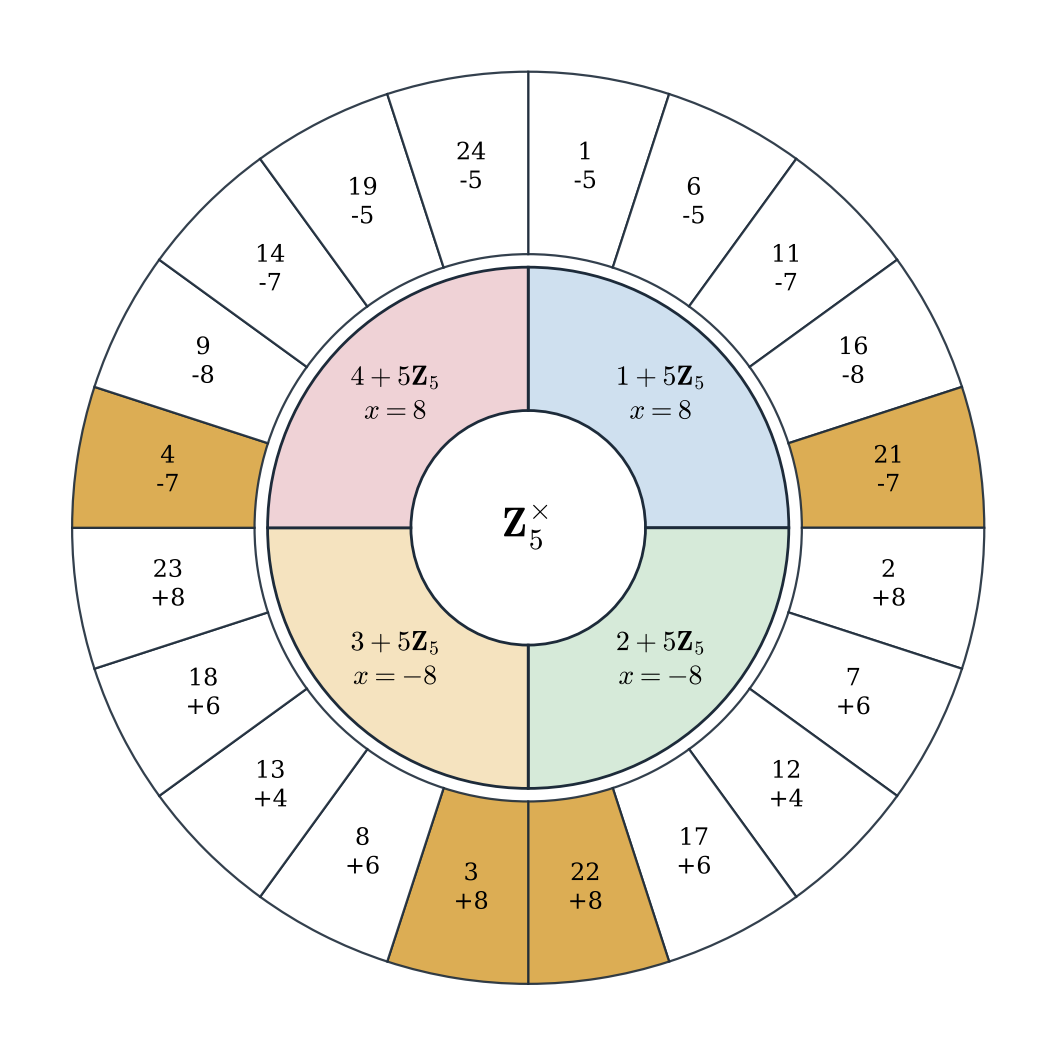
\includegraphics[width=0.6\textwidth]{figures/fig_balls.png}
\caption{The classes $b+25\Z_5$ of $\Z_5^\times$, grouped by $b\bmod 5$, for $E_4$. Each outer cell shows $b$ and $2[b/25]^+$; each inner cell shows $2[a/5]^+$. The four shaded classes $\omega(a)\cdot6^4$ give the coefficient of $T^4$.}\label{fig:balls}
\end{figure}

\emph{The regulator.} The unit root is $\alpha=1+3\cdot5+2\cdot5^2+O(5^3)$, so $1-\alpha^{-1}=(\alpha-1)/\alpha\equiv3\cdot5\pmod{5^2}$ and
\[
(1-\alpha^{-1})^2=4\cdot5^2+4\cdot5^3+O(5^4).
\]
The $5$-adic regulator of the four points and the logarithm of the generator are
\[
\Reg_5(P_1,\dots,P_4)=2\cdot5^2+2\cdot5^3+O(5^5),\qquad\log_5(6)=5+2\cdot5^2+4\cdot5^3+O(5^4),
\]
so $\Reg_\gamma=\Reg_5/\log_5(6)^4=2\cdot5^{-2}+5^{-1}+O(1)$, and
\[
S_5=(1-\alpha^{-1})^2\cdot2\cdot\Reg_\gamma=1+2\cdot5+O(5^2).
\]
The factor $5^2$ coming from the anomalous reduction is cancelled exactly by the denominator $5^{-2}$ of the normalised regulator.

\emph{Saturation.} With $\mathcal L=\{13,23,59,67\}$ Proposition~\ref{prop:sat} applies; the vectors are computed in Appendix~\ref{app:sat}.

\emph{Conclusion.} $v_5(a_4)=0=v_5(S_5)$, so Theorem~\ref{thm:criterion} gives $\rk E_4(\Q)=4$, $\Sha(E_4/\Q)[5^\infty]=0$, $\ord_TL_5(E_4,T)=4$, $\Reg_5(E_4/\Q)\ne0$, and the main conjecture for $(E_4,5)$. As a further check, $a_4\equiv S_5\pmod 5$, which is what the $p$-adic leading-term conjecture predicts if $\Sha(E_4/\Q)$ is trivial.

\subsection{The other ordinary primes}
The same steps were carried out for each of the $163$ good ordinary primes $5\le p<1000$; the supersingular primes in this range are $59$, $101$ and $337$. For each $p$, a surjectivity witness $(q_1,q_2,q_3)$ was found (Table~\ref{tab:rank4}), the points were shown to be $p$-saturated by Proposition~\ref{prop:sat}, and $a_4$ was computed from \eqref{eq:closed}. For $161$ of the primes, $v_p(S_p)=0$ and $a_4\not\equiv0\pmod p$. The remaining two, $p=7$ and $p=157$, are irregular: $v_p(\Reg_\gamma)=1$ while $p$ is not anomalous, so $v_p(S_p)=1$. There Proposition~\ref{prop:precision} with $n=3$ gives
\[
a_4\equiv3\cdot7\pmod{7^2},\qquad a_4\equiv34\cdot157\pmod{157^2},
\]
so $v_p(a_4)=1=v_p(S_p)$ in both cases. At each of the $161$ primes with $v_p(S_p)=0$ the residue of $a_4/S_p$ modulo $p$ is $1$. Theorem~\ref{thm:criterion} applies at all of them.

The prime $7$ shows what an irregular prime looks like in practice. Here $a_7=-5$, so $\#\tilde E_4(\F_7)=13$ and $7$ is not anomalous, and $\prod c_v=2$ is a unit. The unit root and the Euler factor are
\[
\alpha=2+2\cdot7+3\cdot7^3+O(7^4),\qquad(1-\alpha^{-1})^2=2+2\cdot7+3\cdot7^2+O(7^3),
\]
both units. The regulator, on the other hand, is divisible by $7^5$ rather than by the $7^4$ that the normalisation removes:
\[
\Reg_7(P_1,\dots,P_4)=6\cdot7^5+4\cdot7^6+O(7^7),\qquad\log_7(8)=7+3\cdot7^2+O(7^3),
\]
so $\Reg_\gamma=6\cdot7+2\cdot7^2+O(7^3)$ and $S_7=3\cdot7+0\cdot7^2+O(7^3)$. At the second level the Riemann sum gives $a_{2,4}\equiv0\pmod7$, which by Proposition~\ref{prop:precision} only says $v_7(a_4)\ge1$ and decides nothing. At the third level, a sum over the $7^2\cdot6=294$ classes of $\Z_7^\times$ modulo $7^3$, or $147$ after the symmetry of Proposition~\ref{prop:leveln}, it gives $a_4\equiv3\cdot7\pmod{7^2}$. So $v_7(a_4)=1=v_7(S_7)$, and the two leading digits agree as well. The witness is $(5,3,3)$, and $\mathcal L=\{3,19,37,79\}$ proves saturation.

\subsection{The supersingular primes}
At a supersingular prime there is no unit root, and the construction of \S\ref{sec:symbols} breaks down: both roots of $X^2-a_pX+p$ have valuation $\tfrac12$ (here $a_p=0$, as $p\ge5$ and $|a_p|<2\sqrt p$ force $a_p=0$ when $p\mid a_p$), and the measure \eqref{eq:mu} with either root is unbounded. Perrin-Riou's remedy is to work in the Dieudonn\'e module $D_p(E)=H^1_{\mathrm{dR}}(E/\Qp)$, a two-dimensional $\Qp$-vector space with basis $\omega,\varphi(\omega)$, where $\varphi$ is Frobenius, normalised to have characteristic polynomial $X^2-p^{-1}a_pX+p^{-1}$. Let $L_{p,\alpha}(E,T)$ be the series of \eqref{eq:Lp} built with a root $\alpha$ in place of the unit root, a power series with coefficients in $\Qp(\alpha)$, and write $L_{p,\alpha}=G+\alpha H$ with $G,H\in\Qp[[T]]$. Following Perrin-Riou \cite[\S3.5]{SW13} put
\[
L_p(E,T)=\bigl(G(T)+a_pH(T)\bigr)\,\omega-p\,H(T)\,\varphi(\omega),
\]
a power series with coefficients in $D_p(E)$, which carries the same information as $L_{p,\alpha}$ and whose coordinates in the basis $\omega,\varphi(\omega)$ do not depend on the Weierstrass model. The $p$-adic height takes values in $D_p(E)$ as well, and so does the regulator $\Reg_p(E/\Q)$. Perrin-Riou's analogue of Theorem~\ref{thm:schneider} and Kato's divisibility combine exactly as in Theorem~\ref{thm:criterion} \cite[Thm.~6.2 and Algorithm~11.1]{SW13}: if the leading coefficients are compared coordinate by coordinate, the bound is
\[
v_p\#\Sha(E/\Q)[p^\infty]\le\ord_p\bigl((1-\varphi)^{-2}L_p^*(E,0)\bigr)-\ord_p\Bigl(\prod_vc_v\cdot\Reg_\gamma(E/\Q)\Bigr),
\]
where $L_p^*(E,0)$ is the coefficient of $T^r$ and $\ord_p$ of an element of $D_p(E)$ is the least valuation of its coordinates.

For $p=59$ and $p=101$ we computed both sides, using the basis $(-9,19)$, $(-8,23)$, $(-7,25)$, $(4,-7)$ of $E_4(\Q)$, which is $p$-saturated at $59$ and $101$ by Proposition~\ref{prop:sat}. At $p=59$ the coordinates are
\begin{align*}
(1-\varphi)^{-2}L_{59}^*(E_4,0)&=\bigl(22+O(59),\ 54\cdot59+O(59^2)\bigr),\\
2\,\Reg_\gamma&=\bigl(22+48\cdot59+O(59^2),\ 54\cdot59+36\cdot59^2+O(59^3)\bigr),
\end{align*}
and at $p=101$
\begin{align*}
(1-\varphi)^{-2}L_{101}^*(E_4,0)&=\bigl(61+O(101),\ 36\cdot101+O(101^2)\bigr),\\
2\,\Reg_\gamma&=\bigl(61+66\cdot101+O(101^2),\ 36\cdot101+14\cdot101^2+O(101^3)\bigr).
\end{align*}
The $L$-values come from the Riemann sums of level $3$, in which the coefficients of $T^0,\dots,T^3$ vanish to the available precision. In both cases both sides have $\ord_p=0$, so the bound is $0$ and $\Sha(E_4/\Q)[59^\infty]=\Sha(E_4/\Q)[101^\infty]=0$. As at the ordinary primes, the coordinates agree beyond their valuations: the first digits coincide in all four. The witnesses $(3,11,3)$ and $(3,5,3)$ show surjectivity at $59$ and $101$.

\subsection{The prime two}
A complete $2$-descent on $E_4$ \cite[\S3.6]{Cre97} gives $\dim_{\F_2}\Sel^{(2)}(E_4/\Q)=4$. Since $E_4(\Q)[2]=0$ and $\rk E_4(\Q)=4$, the exact sequence $0\to E_4(\Q)/2E_4(\Q)\to\Sel^{(2)}(E_4/\Q)\to\Sha(E_4/\Q)[2]\to0$ forces $\Sha(E_4/\Q)[2]=0$. This completes the proof of Theorem~\ref{thm:A}.

The primes $3$ and $337$ are not covered: $p=3$ is excluded by the hypothesis $p\ge5$ of Theorem~\ref{thm:kato} as used here, and at $p=337$ the Riemann sums for the supersingular $L$-function were too large to evaluate.

\section{Rank three}\label{sec:rank3}

\subsection{The range}
Cremona's tables list \NBcurves{} curves of rank three with conductor $30\,000<N\le100\,000$, in \NBclasses{} isogeny classes, together with three independent points on each. None has complex multiplication. For each class we take the first curve $E$ and each prime $5\le p<100$ of good ordinary reduction, \NBtotal{} pairs in all. By Proposition~\ref{prop:isogeny} the conclusions transfer to the other curves of the class.

\subsection{Proof of Theorem~\ref{thm:B}}
For each pair:
\begin{enumerate}
\item a surjectivity witness exists, so $\rhobar$ is surjective (no pair failed);
\item the three points are $p$-saturated, by Proposition~\ref{prop:sat};
\item $S_p$ and $a_3$ were computed, $a_3$ by \eqref{eq:closed}.
\end{enumerate}
For \NBregular{} pairs, $v_p(S_p)=0$ and $a_3\not\equiv0\pmod p$, so \eqref{eq:test} holds at the second level. The remaining \NBirregular{} pairs all have $v_p(S_p)>0$; for them the precision of the second level is not enough, and the Riemann sums of higher level were evaluated. By Proposition~\ref{prop:precision}, a pair with $v_p(S_p)=v$ can be settled at level $v+2$ and no lower, since $a_{n,3}$ determines $a_3$ only modulo $p^{n-1}$. Level $v+2$ sufficed in every case: there are \NBlevelthree{} pairs with $v=1$, \NBlevelfour{} with $v=2$ and \NBlevelfive{} with $v=3$, and for each of them $v_p(a_3)=v$; the pairs with $v\ge2$ are listed in Table~\ref{tab:deep}. Figure~\ref{fig:levels} shows how the pairs are spread over primes and levels: the deeper levels are needed almost only at the small primes, where the sums are cheap. The most expensive pair is $(60803a1,89)$, where $v_{89}(S_{89})=2$ and $a_3\equiv84\cdot89^2\pmod{89^3}$ required the sum $L_{89,4}$, with about $3.1\cdot10^7$ modular symbols of denominator $89^4$ after the symmetry $[-r]^+=[r]^+$ is used. Thus \eqref{eq:test} holds for all \NBtotal{} pairs, and Theorem~\ref{thm:criterion} gives Theorem~\ref{thm:B}. At each of the \NBregular{} pairs settled at the second level, the residue of $a_3/S_p$ modulo $p$ is $1$.

Since every class contains a pair to which Theorem~\ref{thm:criterion} applies, $\rk E(\Q)=3$ for every curve in the range.

\begin{figure}[t]
\centering
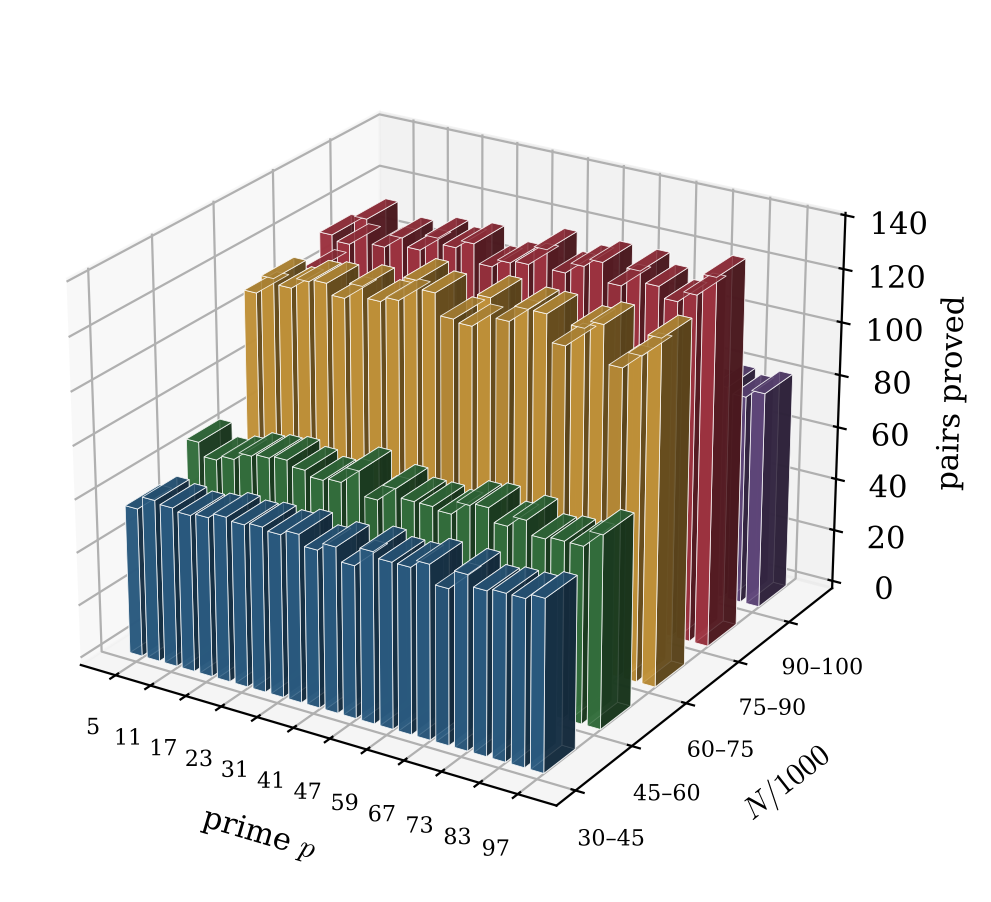
\includegraphics[width=0.86\textwidth]{figures/fig_rank3_bars.png}
\caption{Pairs $(E,p)$ settled in Theorem~\ref{thm:B}, by prime and by conductor.}\label{fig:rank3}
\end{figure}

\begin{figure}[t]
\centering
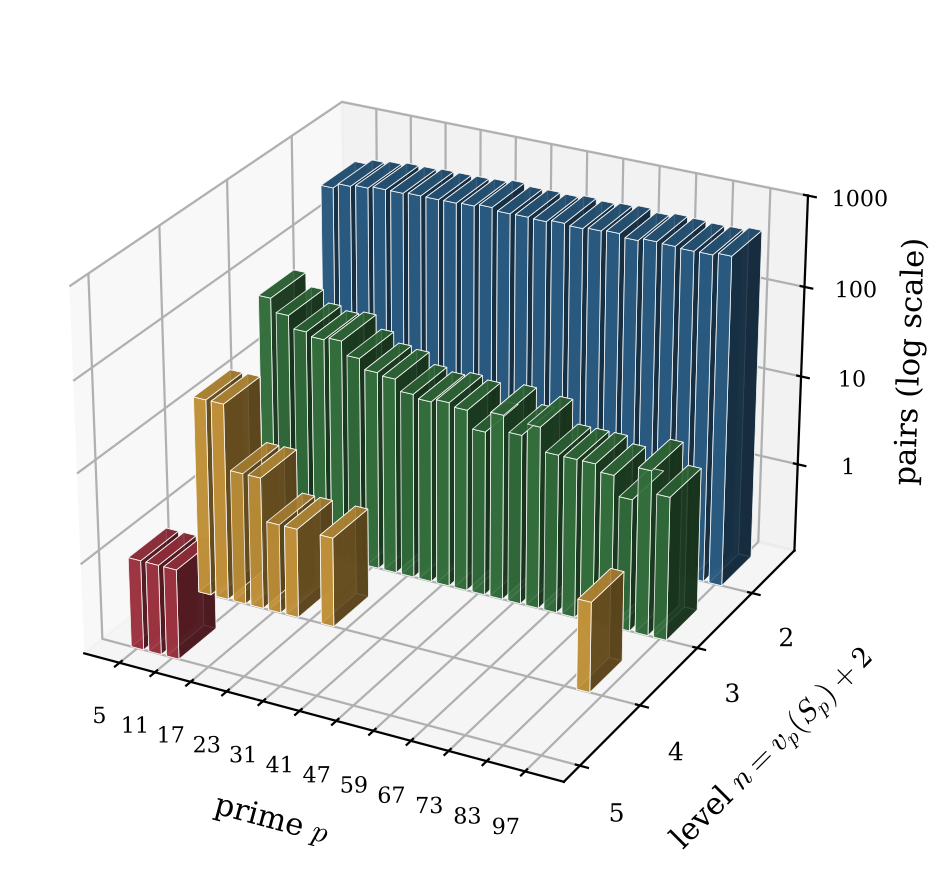
\includegraphics[width=0.8\textwidth]{figures/fig_levels.png}
\caption{The level $n$ of the Riemann sum at which each rank-three pair is settled, by prime, on a logarithmic scale. A pair with $v_p(S_p)=v$ is settled at level $v+2$ and at no lower level.}\label{fig:levels}
\end{figure}

\subsection{Two irregular pairs}\label{ssec:irregex}
Two examples show how the deeper sums settle irregular pairs. In both, the Riemann sum of the second level returns $a_{2,3}\equiv0\pmod p$, which is consistent with any $v_p(a_3)\ge1$ and decides nothing.

\emph{The curve $30446a1$ at $p=5$.} The minimal model is $y^2+xy=x^3+x^2-39x-59$, with conductor $2\cdot13\cdot1171$, discriminant $2^4\cdot13^2\cdot1171$, $\prod c_v=4$ and trivial torsion; the points
\[
P_1=(-3,8),\qquad P_2=(10,21),\qquad P_3=(-5,9)
\]
are independent. Here $a_5=-3$, $\#\tilde E(\F_5)=9$, and
\[
\alpha=2+5+5^2+3\cdot5^3+O(5^4),\qquad(1-\alpha^{-1})^2=4+2\cdot5+O(5^3).
\]
Modulo $5^4$ the height pairing on $P_1,P_2,P_3$ is
\[
\bigl(\langle P_i,P_j\rangle_5\bigr)\equiv\begin{pmatrix}300&175&30\\175&325&450\\30&450&30\end{pmatrix}\pmod{5^4},
\]
every entry divisible by $5$. Since the entries are known to an error of $5^4$ and have valuation at least $1$, the determinant is known modulo $5^6$, and it is $1250=2\cdot5^4$. So $\Reg_5=2\cdot5^4+0\cdot5^5+O(5^6)$, and with $\log_5(6)=5+2\cdot5^2+4\cdot5^3+O(5^4)$,
\[
\Reg_\gamma=\frac{\Reg_5}{\log_5(6)^3}=2\cdot5+3\cdot5^2+O(5^3),\qquad S_5=(1-\alpha^{-1})^2\cdot4\cdot\Reg_\gamma=2\cdot5+0\cdot5^2+O(5^3).
\]
The prime $5$ is not anomalous and divides no Tamagawa number; the irregularity comes entirely from the regulator, which is divisible by $5^4$ instead of $5^3$. The sum of the third level runs over the $100$ classes of $\Z_5^\times$ modulo $5^3$, or $50$ after the symmetry of Proposition~\ref{prop:leveln}, and gives $a_3\equiv2\cdot5\pmod{5^2}$. So $v_5(a_3)=1=v_5(S_5)$, and the leading digits agree. With the witness $(17,3,17)$ and $\mathcal L=\{3,11,31\}$, Theorem~\ref{thm:criterion} gives $\Sha(E/\Q)[5^\infty]=0$.

\emph{The curve $60803a1$ at $p=89$.} The minimal model is $y^2+y=x^3+x^2-65x+195$, with conductor $41\cdot1483$, discriminant $-41^2\cdot1483$, $\prod c_v=2$ and trivial torsion; the points are
\[
P_1=(-5,20),\qquad P_2=\bigl(\tfrac{21}{4},\tfrac{37}{8}\bigr),\qquad P_3=\bigl(\tfrac{37}{9},\tfrac{89}{27}\bigr).
\]
Here $a_{89}=-12$ and $\#\tilde E(\F_{89})=102$, so again only the regulator contributes:
\[
\alpha=77+51\cdot89+O(89^2),\qquad(1-\alpha^{-1})^2=50+47\cdot89+O(89^2),
\]
\[
\Reg_{89}=40\cdot89^5+41\cdot89^6+O(89^7),\qquad\log_{89}(90)=89+44\cdot89^2+O(89^3),
\]
so $\Reg_\gamma=40\cdot89^2+12\cdot89^3+O(89^4)$ and
\[
S_{89}=84\cdot89^2+20\cdot89^3+O(89^4).
\]
This is the only pair with $p\ge29$ and $v_p(S_p)=2$. By Proposition~\ref{prop:precision} the coefficient $a_3$ is determined modulo $89^{n-1}$ by the sum of level $n$, so level $4$ is the first that can see $v_{89}(a_3)=2$. The third level returns $0$ modulo $89^2$; the fourth needs $[b/89^4]^+$ for $88\cdot89^3/2\approx3.1\cdot10^7$ classes $b$ and gives
\[
a_3\equiv84\cdot89^2\pmod{89^3}.
\]
The witness is $(7,3,3)$ and $\mathcal L=\{79,269,983\}$, so Theorem~\ref{thm:criterion} gives $\Sha(E/\Q)[89^\infty]=0$ for every curve in the isogeny class $60803a$.

In both examples the first nonzero digit of $a_3$ equals that of $S_p$. This is the congruence $a_r\equiv S_p$ modulo $p^{v_p(S_p)+1}$ which the $p$-adic leading-term formula predicts once $\Sha(E/\Q)[p^\infty]=0$; it is not used in the proofs, but it holds for all \NBirregular{} irregular rank-three pairs, as well as for $E_4$ at $7$ and $157$.

\subsection{How often a prime is irregular}
A pair is irregular when $v_p(S_p)>0$. Three quantities contribute to $v_p(S_p)$: the Euler factor, of valuation $2v_p(\#\tilde E(\F_p))$; the Tamagawa product; and the normalised regulator $\Reg_\gamma$, whose valuation can be negative. They are not independent. At an anomalous prime the Euler factor has valuation $2$, but the regulator usually compensates: of the $320$ anomalous pairs in the range, $285$ are regular, with $v_p(\Reg_\gamma)=-2$, as for $E_4$ at $5$. Remark~\ref{rem:integral} explains why the total is never negative once $\Sha(E/\Q)[p^\infty]$ is known to vanish. If the residues of these quantities modulo $p$ behaved like random elements of $\F_p$, a fixed $p$ would be irregular for a proportion of curves close to $c/p$ for a constant $c$. Figure~\ref{fig:irregular} shows $p$ times the observed proportion, and Table~\ref{tab:primes} lists the counts. The product stays between $0.55$ and $1.55$ across the whole range, with mean \NBirrmean, so the proportion of irregular pairs at $p$ falls off like $1/p$, as the random model predicts. The irregular pairs are the expensive ones, since they need Riemann sums at the third or fourth level, and their number therefore drops quickly as $p$ grows.

\begin{figure}[t]
\centering
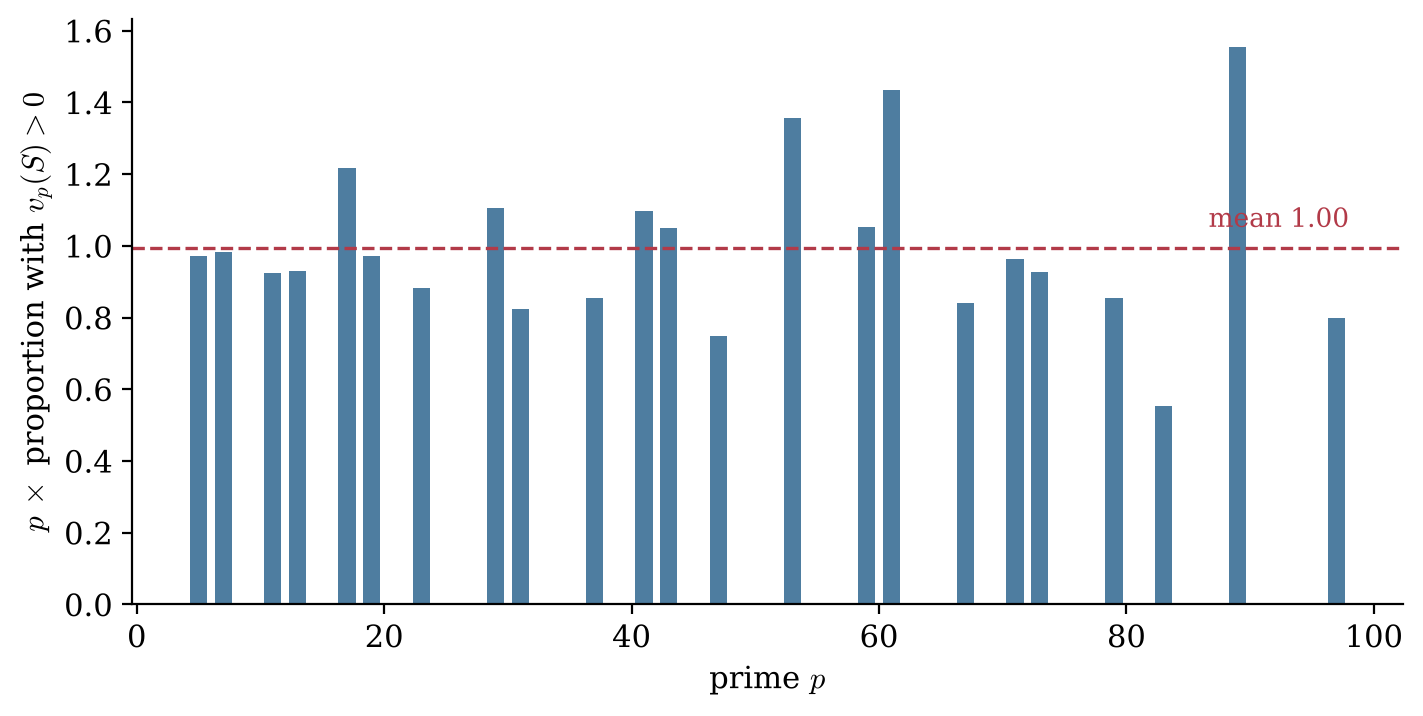
\includegraphics[width=0.82\textwidth]{figures/fig_irregular.png}
\caption{For each prime $p<100$, $p$ times the proportion of the rank-three pairs with $v_p(S_p)>0$.}\label{fig:irregular}
\end{figure}

\section{Ranks five and six}\label{sec:rank56}

\subsection{The curves}
$E_5$ has prime conductor $19\,047\,851$ and discriminant $-19\,047\,851$, so its reduction at the conductor is of type $\mathrm{I}_1$, $\prod c_v=1$ and $E_5(\R)$ is connected. $E_6$ has discriminant $2^2\cdot3^2\cdot2777\cdot311\,341$, reduction of type $\mathrm I_2$ at $2$ and $3$ and $\mathrm I_1$ at the other two primes, $\prod c_v=4$, and two real components. Both curves are semistable. Their torsion is trivial: for $E_5$ the orders $\#\tilde E_5(\F_3)=7$ and $\#\tilde E_5(\F_5)=9$ are coprime; for $E_6$ the orders $10,12,18,20$ at $5,7,11,13$ have greatest common divisor $2$, and $E_6(\Q)[2]=0$ by the irreducibility witness $q=17$, $a_{17}=-7$. Irreducibility witnesses exist for all twelve primes of Mazur's list, so neither curve has a rational isogeny; in particular each is the optimal curve of its class, and its Manin constant is $1$ by \v{C}esnavi\v{c}ius' theorem for semistable curves \cite{Ces18}.

The points
\[
E_5\colon\ (-10,11),\ (-\tfrac{39}{4},\tfrac{105}{8}),\ (-8,21),\ (-7,23),\ (-6,24),
\]
\[
E_6\colon\ (-59,35),\ (-58,116),\ (-\tfrac{229}{4},\tfrac{1141}{8}),\ (-53,227),\ (-\tfrac{193}{4},\tfrac{2215}{8}),\ (32,-4)
\]
lie on the curves and are $p$-saturated at every prime $p<100$ by Proposition~\ref{prop:sat}.

\subsection{Modular symbols at large conductor}
At these conductors the space of modular symbols is too large for the linear-algebra method of \cite{Cre97}. The values $[r]^+$ were instead computed by Wuthrich's numerical method \cite{Wut18}: the integral $\lambda^+(r)$ is evaluated from the Fourier expansion of $f$ at a suitable cusp, with a rigorous bound for the error, and rounded to the unique rational number with the known denominator. The denominator bound is the one in the proof of Lemma~\ref{lem:symbols}(c), with $c=1$; this is where the value of the Manin constant enters.\footnote{This is the only place where the Manin constant itself, and not merely its integrality, is used; \cite{Wut18} states the requirement explicitly.}

\subsection{The prime seven for \texorpdfstring{$E_5$}{E5}}\label{ssec:e5p7}
As for $E_4$ at $5$, every step can be followed by hand. Here $a_7=-4$, so $7$ is good ordinary, $\#\tilde E_5(\F_7)=12$, and $7$ divides no Tamagawa number. By Lemma~\ref{lem:heightval} the regulator $\Reg_\gamma$ is a $7$-adic integer, and the unit root of $X^2+4X+7$ is
\[
\alpha=3+7+6\cdot7^2+O(7^3),\qquad 1-\alpha^{-1}\equiv1-5\equiv3\pmod7,
\]
so $(1-\alpha^{-1})^2$ is a unit. With the five points of the previous subsection,
\[
\Reg_7=2\cdot7^5+6\cdot7^6+4\cdot7^7+O(7^8),\qquad S_7(E_5)=(1-\alpha^{-1})^2\,\Reg_\gamma=4+5\cdot7+4\cdot7^2+O(7^3).
\]
Every entry of the $5\times5$ height matrix is divisible by $7$, as Lemma~\ref{lem:heightval} predicts, and its determinant is divisible by $7^5$ and by no higher power: the pair is regular.

For the Riemann sum, \eqref{eq:closed} with $k=5$ involves only $j=5$ and $j=6$, with $\binom55=1$ and $\binom65=6$. All six symbols $[a/7]^+$ vanish, so only the symbols of denominator $49$ contribute:
\[
\begin{array}{c|cccccc}
a&1&2&3&4&5&6\\\hline
b_{a,5}&36&2&38&11&47&13\\
{}[b_{a,5}/49]^+&1&-1&0&0&-1&1\\\hline
b_{a,6}&43&16&10&39&33&6\\
{}[b_{a,6}/49]^+&1&1&1&1&1&1
\end{array}
\]
The symmetry $[-r]^+=[r]^+$ is visible in the pairs $b+b'=49$. Since $a_7\equiv3$ and $3^{-2}\equiv4\pmod 7$,
\[
a_5\equiv4\bigl((1-1+0+0-1+1)+6\cdot(1+1+1+1+1+1)\bigr)=144\equiv4\pmod7,
\]
which is the first digit of $S_7(E_5)$. The same computation with $k\le4$ gives $a_0\equiv\cdots\equiv a_4\equiv0$. So $v_7(a_5)=v_7(S_7)=0$, and with the witness $(2,3,3)$ Theorem~\ref{thm:criterion} gives $\rk E_5(\Q)=5$ and $\Sha(E_5/\Q)[7^\infty]=0$.

One level higher the agreement persists. Proposition~\ref{prop:leveln} with $n=3$ uses the $168$ symbols of denominators $49$ and $343$ that remain after the symmetry, and gives
\[
a_0\equiv\cdots\equiv a_4\equiv0,\qquad a_5\equiv39=4+5\cdot7\pmod{7^2},
\]
so the first two digits of $a_5$ and of $S_7(E_5)$ coincide. This is what the $p$-adic conjecture of Mazur, Tate and Teitelbaum predicts once $\Sha(E_5/\Q)[7^\infty]=0$ is known (Section~\ref{sec:leading}).

\subsection{Proof of Theorems~\ref{thm:C} and~\ref{thm:D}}
For $E_5$ and $p=7,11,13,17,19$ all pairs are regular, $v_p(S_p)=0$, and \eqref{eq:closed} gives
\[
a_5\equiv4,\ 2,\ 7,\ 13,\ 16\pmod{p}\quad\text{for } p=7,11,13,17,19 .
\]
The surjectivity witnesses are $(2,3,3)$, $(2,17,3)$, $(5,2,3)$, $(3,2,3)$, $(2,3,3)$. Theorem~\ref{thm:criterion} applies at each of these primes.\RfivePfive

For $E_6$ and $p=7$, the witness $(5,19,5)$ shows surjectivity, $v_7(S_7)=0$, and \eqref{eq:closed} with $k=6$ gives $a_6\equiv6\pmod7$, with $a_0,\dots,a_5\equiv0$. Theorem~\ref{thm:criterion} applies. In all six cases $a_r\equiv S_p\pmod p$.

The primes $5$ for $E_5$ (where $v_5(S_5)=1$) and $p\ge11$ for $E_6$, and $p\ge23$ for $E_5$, are left open: the Riemann sums at these primes require modular symbols with denominators $p^2$ or $p^3$, and their evaluation at these conductors exceeded the computation we could carry out.

\section{The leading coefficient}\label{sec:leading}

Theorem~\ref{thm:criterion} compares the valuations of two numbers, the coefficient $a_r$ of $T^r$ in $L_p(E,T)$ and
\[
S_p(E)=\Bigl(1-\frac1\alpha\Bigr)^2\,\frac{\prod_vc_v\cdot\Reg_\gamma(E/\Q)}{\#E(\Q)_\tors^2},
\]
and it uses nothing beyond the valuations. The $p$-adic conjecture of Mazur, Tate and Teitelbaum \cite{MTT86}, in the form of \cite{SW13} for good ordinary $p$, predicts the numbers themselves: if $\Sha(E/\Q)$ is finite, then
\begin{equation}\label{eq:mtt}
a_r=\#\Sha(E/\Q)\cdot S_p(E).
\end{equation}
Theorem~\ref{thm:criterion} proves the $p$-part of this identity, $v_p(a_r)=v_p(S_p)$ together with $v_p\#\Sha(E/\Q)=0$. The remaining content of \eqref{eq:mtt} at a pair where $\Sha[p^\infty]=0$ is a congruence between $a_r$ and $S_p$ beyond their common valuation, and it can be tested by the same Riemann sums one level higher.

\begin{proposition}\label{prop:leading}
Let $(E,p)$ be one of the \NLpairs{} pairs of Theorem~\ref{thm:B} with $p\in\{5,7,11,13\}$, and let $v=v_p(S_p(E))$. Then
\[
a_3\equiv S_p(E)\pmod{p^{v+2}} .
\]
Consequently, if $\Sha(E/\Q)$ is finite, then \eqref{eq:mtt} holds modulo $p^{v+2}$ if and only if $\#\Sha(E/\Q)\equiv1\pmod{p^2}$.
\end{proposition}

\begin{proof}
For each pair, Proposition~\ref{prop:leveln} with $n=v+3$ gives $a_3$ modulo $p^{v+2}$, since $3<p$; the symbols needed have denominators $p^{v+2}$ and $p^{v+3}$. The regulator is computed to $p$-adic precision $p^{v+8}$ by the method of \S\ref{ssec:heightcomp}; after division by $\log_p(1+p)^3$, of valuation $3$, this determines $S_p$ modulo $p^{v+2}$ with room to spare. The two residues coincide in every case. For the second statement write $S_p=p^vu$ with $u\in\Zp^\times$; then $\#\Sha\cdot S_p-a_3\equiv(\#\Sha-1)p^vu\pmod{p^{v+2}}$, which vanishes modulo $p^{v+2}$ exactly when $p^2\mid\#\Sha-1$.
\end{proof}

The congruence of Proposition~\ref{prop:leading} is an independent test: Theorem~\ref{thm:criterion} only needed the first $p$-adic digits of $a_3$ and $S_p$ to be nonzero, while the proposition matches their first two digits. If the second digits were unrelated, each pair would pass with probability $1/p$, and the \NLpairs{} pairs together would pass with probability below $5^{-\NLpairsfive}$. Figure~\ref{fig:leading} shows the second digits at $p=7$ and $p=13$: they are spread over all residues, and every pair sits on the diagonal. Table~\ref{tab:leading} lists the pairs with $v\ge2$, where the congruence holds modulo $p^4$, and in three cases modulo $p^5$.

The classical side gives the expected value of $\#\Sha$. For the first curve of each of the $8\,862$ isogeny classes of rank three with conductor between $30\,000$ and $500\,000$ in Cremona's tables, the number
\[
\#\Sha_{\mathrm{an}}(E/\Q)=\frac{L^{(3)}(E,1)}{3!}\cdot\frac{\#E(\Q)_\tors^2}{\Omega_E\prod_vc_v\Reg(E/\Q)},
\]
computed from the generators in the tables with the real height pairing, is $1$ to within $10^{-15}$; the same holds for $E_4$, $E_5$ and $E_6$ with the derivatives of order four, five and six.\footnote{This is a numerical computation of $L^{(r)}(E,1)$ by the rapidly converging series of the functional equation; it is not a proof that $L^{(r)}(E,1)$ has the computed value, and none of the theorems of this paper depends on it.} So the classical conjecture predicts $\#\Sha(E/\Q)=1$, \eqref{eq:mtt} becomes $a_r=S_p$, and Proposition~\ref{prop:leading} is this identity modulo $p^{v+2}$, proved for every pair it covers. For $E_5$ at $7$ the first two digits of $a_5$ and $S_7$ agree by \S\ref{ssec:e5p7}, and for $E_4$ at its two irregular primes $7$ and $157$ the first digits agree by the computation at level three in \S\ref{sec:rank4}.

\begin{figure}[t]
\centering
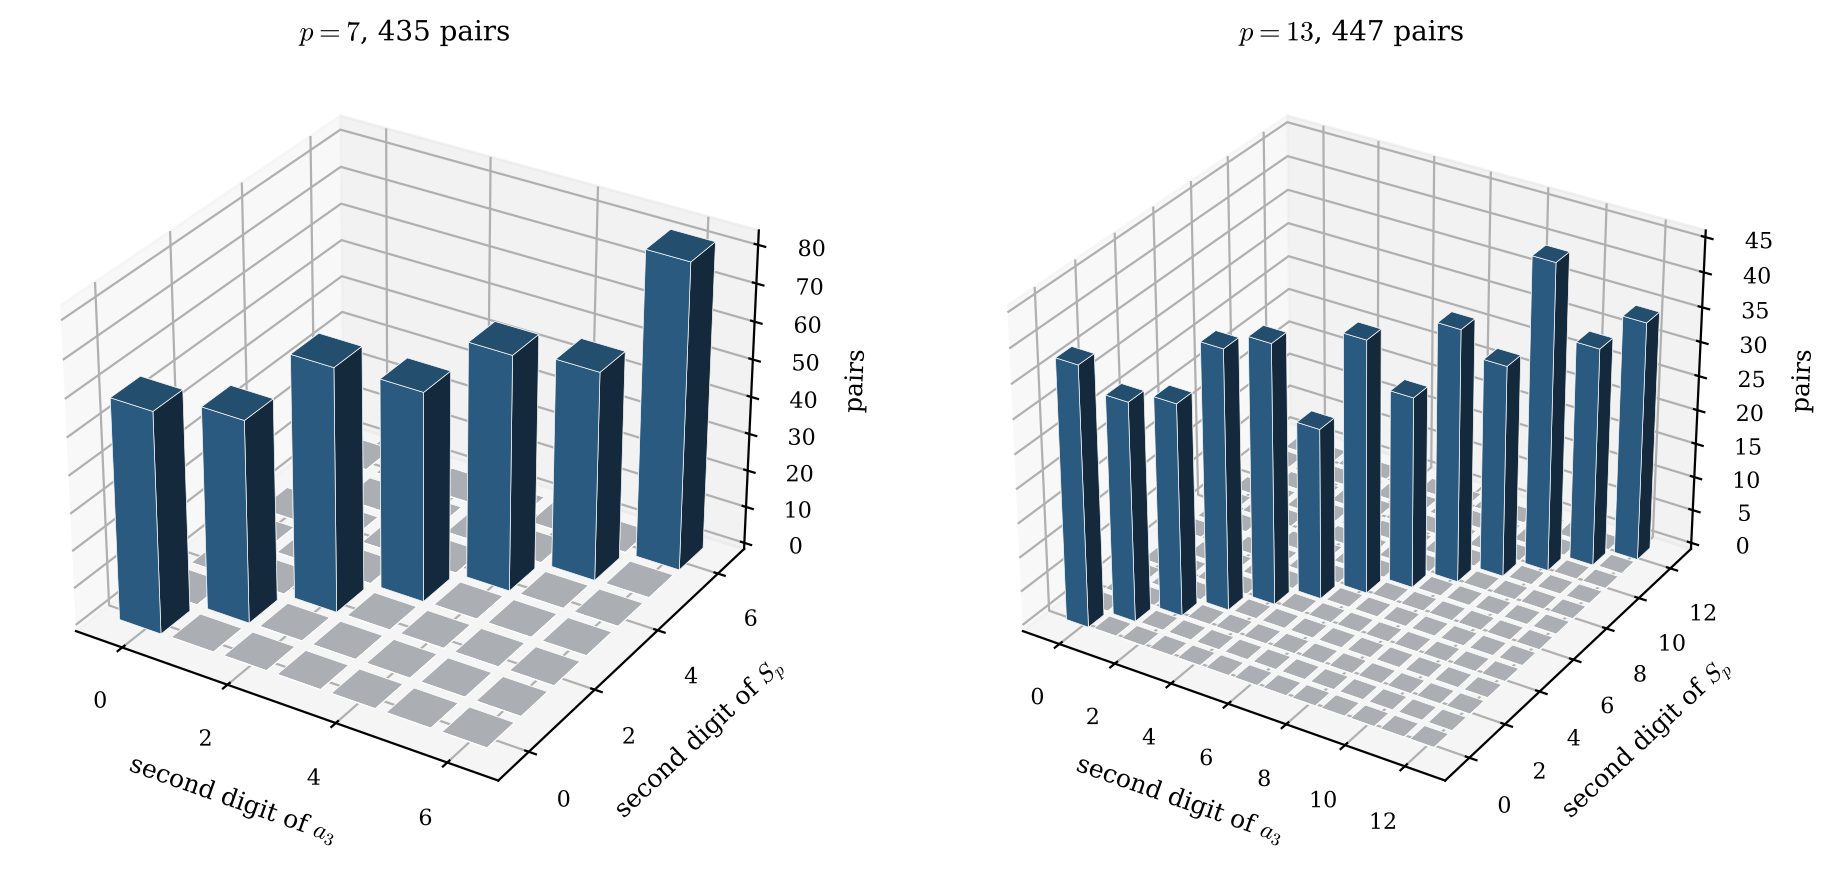
\includegraphics[width=\textwidth]{figures/fig_leading.png}
\caption{The digit of $p^{v+1}$ in $a_3$ and in $S_p$, where $v=v_p(S_p)$, for the pairs of Proposition~\ref{prop:leading} at $p=7$ and $p=13$. Grey tiles are empty cells; all pairs lie on the diagonal.}\label{fig:leading}
\end{figure}

\begin{table}[t]
\centering\small
\caption{The pairs of Proposition~\ref{prop:leading} with $v_p(S_p)\ge2$: the common residue of $a_3$ and $S_p$ modulo $p^{v+2}$, written in base $p$ from the digit of $p^v$.}\label{tab:leading}
\begin{tabular}{lrrl@{\qquad}lrrl}
\hline
curve & $p$ & $v$ & $a_3\equiv S_p$ & curve & $p$ & $v$ & $a_3\equiv S_p$\\
\hline
33609a1 & 11 & 2 & $10\cdot11^{2}+2\cdot11^{3}$ & 73931a1 & 7 & 2 & $5\cdot7^{2}$\\
38600m1 & 7 & 2 & $7^{2}+7^{3}$ & 74216a1 & 5 & 2 & $4\cdot5^{2}+3\cdot5^{3}$\\
43556b1 & 5 & 2 & $5^{2}+5^{3}$ & 74434a1 & 5 & 2 & $2\cdot5^{2}+4\cdot5^{3}$\\
45352a1 & 5 & 2 & $3\cdot5^{2}+2\cdot5^{3}$ & 74864b1 & 7 & 2 & $2\cdot7^{2}+4\cdot7^{3}$\\
47087a1 & 5 & 2 & $4\cdot5^{2}+4\cdot5^{3}$ & 78287b1 & 7 & 2 & $2\cdot7^{2}+4\cdot7^{3}$\\
47696h1 & 5 & 2 & $2\cdot5^{2}$ & 80256a1 & 5 & 2 & $4\cdot5^{2}+4\cdot5^{3}$\\
49411a1 & 5 & 2 & $3\cdot5^{2}+3\cdot5^{3}$ & 81328c1 & 7 & 2 & $4\cdot7^{2}+6\cdot7^{3}$\\
49626a1 & 7 & 2 & $4\cdot7^{2}+3\cdot7^{3}$ & 83928b1 & 5 & 2 & $3\cdot5^{2}+3\cdot5^{3}$\\
51052a1 & 7 & 2 & $4\cdot7^{2}+7^{3}$ & 87866a1 & 5 & 2 & $5^{2}+2\cdot5^{3}$\\
53122a1 & 5 & 3 & $5^{3}+2\cdot5^{4}$ & 88022a1 & 7 & 2 & $4\cdot7^{2}+5\cdot7^{3}$\\
53122a1 & 7 & 2 & $3\cdot7^{2}+6\cdot7^{3}$ & 88502f1 & 5 & 2 & $3\cdot5^{2}+2\cdot5^{3}$\\
53957b1 & 5 & 2 & $2\cdot5^{2}+5^{3}$ & 88883a1 & 7 & 2 & $5\cdot7^{2}+6\cdot7^{3}$\\
54489b1 & 7 & 2 & $4\cdot7^{2}+2\cdot7^{3}$ & 89294a1 & 11 & 3 & $5\cdot11^{3}+3\cdot11^{4}$\\
59450i1 & 7 & 2 & $5\cdot7^{2}+2\cdot7^{3}$ & 90953a1 & 7 & 3 & $7^{3}$\\
61886d1 & 7 & 2 & $4\cdot7^{2}+7^{3}$ & 91506a1 & 5 & 2 & $2\cdot5^{2}+2\cdot5^{3}$\\
62576b1 & 13 & 2 & $12\cdot13^{2}$ & 91958a1 & 5 & 2 & $4\cdot5^{2}+3\cdot5^{3}$\\
63574d1 & 5 & 2 & $2\cdot5^{2}$ & 92651a1 & 11 & 2 & $5\cdot11^{2}+10\cdot11^{3}$\\
65122e1 & 7 & 2 & $5\cdot7^{2}+7^{3}$ & 94281b1 & 5 & 2 & $2\cdot5^{2}+4\cdot5^{3}$\\
67064a1 & 11 & 2 & $6\cdot11^{2}$ & 97111a1 & 13 & 2 & $2\cdot13^{2}+13^{3}$\\
70449b1 & 7 & 2 & $6\cdot7^{2}$ & 98231a1 & 13 & 2 & $6\cdot13^{2}+10\cdot13^{3}$\\
71688a1 & 7 & 2 & $7^{2}+6\cdot7^{3}$ &  &  &  & \\
\hline
\end{tabular}

\end{table}

Two remarks put this in context. First, \eqref{eq:mtt} is not known for a single curve of rank at least two, since it presupposes the finiteness of $\Sha(E/\Q)$; what can be proved, here and in \cite{SW13}, is its $p$-part at explicit pairs. Second, the proposition does not depend on $\#\Sha_{\mathrm{an}}$, which enters only in its interpretation; what is proved is the congruence between the two explicit $p$-adic numbers $a_3$ and $S_p$.

\section{From the \texorpdfstring{$p$}{p}-parts to the conjecture}\label{sec:gap}

Theorem~\ref{thm:criterion} treats one prime at a time and says nothing about $L(E,s)$ at $s=1$. This section sets out precisely what separates the results of this paper from the conjecture \eqref{eq:bsd} for the same curves, because the missing pieces are of different kinds: one concerns the complex $L$-function, one concerns infinitely many primes, and one concerns the comparison of the $p$-adic and complex sides.

\subsection{The analytic rank}
The order of vanishing of $L(E,s)$ at $s=1$ can be bounded above by a computation: a single value $L^{(k)}(E,1)$ shown to be nonzero with a rigorous error bound gives $\ord_{s=1}L(E,s)\le k$. Bounding it below is harder, since a vanishing derivative cannot be recognised numerically. Two exact tools are available. The global root number $w(E)=\pm1$, the sign in the functional equation of $L(E,s)$, equals $(-1)^{\ord_{s=1}L(E,s)}$ and is computed exactly as a product of local root numbers \cite{Cre97}. And the theorems of Gross--Zagier and Kolyvagin determine the rank when the analytic rank is at most one. Combined with the results of this paper they give a lower bound.

\begin{corollary}\label{cor:analytic}
For every curve $E$ of Theorem~\ref{thm:B} and for $E_5$, $\ord_{s=1}L(E,s)$ is odd and at least $3$. For $E_4$ and $E_6$ it is even and at least $2$.
\end{corollary}

\begin{proof}
Let $m=\ord_{s=1}L(E,s)$. If $m\le1$, then $\rk E(\Q)=m$ by the formula of Gross and Zagier \cite{GZ86} and Kolyvagin's Euler system \cite{Kol90}, with the auxiliary imaginary quadratic field supplied by the nonvanishing theorems of Bump, Friedberg and Hoffstein \cite{BFH90} and of Murty and Murty \cite{MM91}. Theorems~\ref{thm:A}--\ref{thm:D} give $\rk E(\Q)\ge3$ in every case, so $m\ge2$. The root number is $-1$ for every curve of Theorem~\ref{thm:B} and for $E_5$, and $+1$ for $E_4$ and $E_6$; so $m$ is odd in the first case and even in the second.
\end{proof}

For the curves of rank three the corollary leaves only the upper bound, which is a matter of showing $L'''(E,1)\ne0$; Buhler, Gross and Zagier \cite{BGZ85} did this with rigorous error control for the curve $5077a1$, the smallest conductor of rank three, and the same evaluation applies to any curve once $L'''(E,1)$ is computed with a certified error. For rank four and higher there is no comparable device. One would need to show $L''(E_4,1)=0$, and no formula expresses $L''(E,1)$ as the height of an algebraic object, so the analytic rank of $E_4$ is known only to be even and at least $2$, while a numerical evaluation gives $L^{(4)}(E_4,1)\approx214.65$, which with a certified error bound would give the upper bound $4$.

\subsection{An upper bound for the Selmer group from \texorpdfstring{$L^{(r)}(E,1)$}{the r-th derivative}}
For $r\le1$ the Euler system of Heegner points bounds the Selmer group \cite{Kol90}, because by the formula of Gross and Zagier the basic Heegner point is of infinite order exactly when $L'(E/K,1)\ne0$. The argument proves finiteness of $\Sha$ for all primes at once. For $r\ge2$ there is no point whose height is $L^{(r)}(E,1)$. Over function fields Yun and Zhang \cite{YZ17} constructed such objects from moduli spaces of shtukas with $r$ legs, and their higher Gross--Zagier formula expresses $L^{(r)}$ as an intersection number; no analogue over $\Q$ is known. Kolyvagin systems of higher rank exist \cite{MR04}, but a theorem that their leading class is nonzero when $L^{(r)}(E,1)\neq0$ is missing.

The method of this paper replaces the complex derivative by the $p$-adic one, and Kato's Euler system supplies the bound that Heegner points supply in rank one. The price is that the $p$-adic statement must be checked one prime at a time: Theorem~\ref{thm:criterion} needs $v_p(a_r)$, which is a property of the particular prime.

\subsection{Infinitely many primes}
To deduce the finiteness of $\Sha(E/\Q)$ from results of the kind proved here one would need Theorem~\ref{thm:criterion} at all but finitely many primes, together with a separate argument at the remaining ones. Three obstacles appear. First, the hypothesis $\rhobar$ surjective fails at finitely many primes by Serre's theorem \cite{Ser72}, and at those the divisibility in Theorem~\ref{thm:kato} holds only up to a power of $p$. Second, half of the primes, in a sense made precise by the Sato--Tate law, are close to supersingular in the relevant range, and the supersingular theory of \S\ref{sec:rank4} is harder to evaluate. Third, and most seriously, the equality $v_p(a_r)=v_p(S_p)$ is a numerical coincidence at each $p$ for which no uniform reason is known. The data of \S\ref{sec:rank3} show that it held without exception, which is what the $p$-adic Birch--Swinnerton-Dyer conjecture predicts if $\Sha(E/\Q)$ is trivial, but a proof for all $p$ would be a proof of that conjecture for $E$.

\subsection{Schneider's conjecture}
Theorem~\ref{thm:criterion} proves $\Reg_p(E/\Q)\ne0$ for each pair it covers, but no argument gives it for all $p$. One route would be a transcendence statement for values of the $p$-adic sigma function at algebraic points, of the kind Bertrand obtained for curves with complex multiplication in rank one. For curves without complex multiplication, and for $r\ge2$, no such statement is known: the regulator is a determinant of $p$-adic logarithms of algebraic points in a formal group, and a vanishing determinant would be an algebraic relation among them.

\subsection{The same order of vanishing for \texorpdfstring{$L_p$}{Lp} and \texorpdfstring{$L$}{L}}
Even if all $p$-adic statements were known, passing from $\ord_TL_p(E,T)=r$ to $\ord_{s=1}L(E,s)=r$ requires a link between derivatives of the two functions. The interpolation property of Proposition~\ref{prop:interp} relates $L_p$ to the values $L(E,\chi,1)$ at finite-order characters, which are central values and not derivatives. For $r=1$ the link is Perrin-Riou's $p$-adic Gross--Zagier formula \cite{PR87}, which expresses $L_p'(E,0)$ through the $p$-adic height of a Heegner point; combined with the complex formula, it shows that the two orders of vanishing agree when one of them is $1$. For $r\ge2$ no such link is known.

\subsection{What is proved}
For each curve and each prime in the stated ranges, the method gives: $\Sha(E/\Q)[p^\infty]$ is trivial, the rank of $E(\Q)$ equals the number of known independent points, the $p$-adic regulator is nonzero, and the main conjecture of Iwasawa theory holds for $(E,p)$. In the language of \eqref{eq:bsd}, the $p$-parts of both sides of the conjectural formula are determined in the $p$-adic setting, and the algebraic side is computed exactly at $p$. These are the parts of the Birch--Swinnerton-Dyer formula that are accessible at present for curves of rank at least two.

\appendix

\section{The error of the Riemann sums}\label{app:precision}

\begin{proof}[Proof of Proposition~\ref{prop:precision}]
For $b=\omega(a)(1+p)^j$ the coefficient $a_{n,k}$ of \eqref{eq:riemann} is $\sum_b\mu(b+p^n\Zp)\binom{j}{k}$, so
\[
a_k-a_{n,k}=\sum_b\int_{b+p^n\Zp}\Bigl(\binom{\ell(x)}{k}-\binom{\ell(b)}{k}\Bigr)d\mu(x).
\]
Let $x\in b+p^n\Zp$. Then $\omega(x)=\omega(b)$, and $\langle x\rangle=\langle b\rangle\,y$ with $y=x/b\in1+p^n\Zp$. Since $\log_p(1+p^n\Zp)=p^n\Zp$ and $v_p(\log_p(1+p))=1$, we have $\ell(x)=j+t$ with $t=\ell(y)\in p^{n-1}\Zp$. By Vandermonde's identity, valid for $p$-adic integers,
\[
\binom{j+t}{k}-\binom{j}{k}=\sum_{i=1}^{k}\binom{j}{k-i}\binom{t}{i},\qquad\binom{t}{i}=\frac{t}{i}\binom{t-1}{i-1}.
\]
The binomial coefficients of $p$-adic integers are $p$-adic integers, so $v_p\binom{t}{i}\ge v_p(t)-v_p(i)\ge n-1-e_k$ for $1\le i\le k$. Thus the integrand takes values in $p^{n-1-e_k}\Zp$, and since $\mu$ is $\Zp$-valued (Lemma~\ref{lem:distribution}), so does each integral.
\end{proof}

\section{Two properties of modular symbols}\label{app:hecke}

\begin{proof}[Proof of Lemma~\ref{lem:symbols}(a) and (b)]
Since $f(\tau+1)=f(\tau)$, the substitution $\tau\mapsto\tau+1$ gives $\lambda(r+1)=\lambda(r)$, hence $[r+1]^+=[r]^+$; and $[-r]^+=[r]^+$ is immediate from the definition.

For (b), the Hecke operator $T_\ell$ with $\ell\nmid N$ acts on weight-two forms by
\[
(T_\ell f)(\tau)=\ell f(\ell\tau)+\frac1\ell\sum_{b=0}^{\ell-1}f\Bigl(\frac{\tau+b}{\ell}\Bigr),
\]
and $T_\ell f=a_\ell f$. Integrate from $r$ to $i\infty$. The substitution $w=\ell\tau$ gives $\int_r^{i\infty}\ell f(\ell\tau)\,d\tau=\int_{\ell r}^{i\infty}f(w)\,dw$, and $w=(\tau+b)/\ell$ gives $\int_r^{i\infty}\frac1\ell f(\frac{\tau+b}\ell)\,d\tau=\int_{(r+b)/\ell}^{i\infty}f(w)\,dw$. Multiplying by $2\pi i$,
\[
a_\ell\lambda(r)=\lambda(\ell r)+\sum_{b=0}^{\ell-1}\lambda\Bigl(\frac{r+b}{\ell}\Bigr).
\]
Applying this to $-r$ and using $\lambda((-r+b)/\ell)=\lambda(-(r+b')/\ell)$ for $b'\equiv-b\pmod\ell$, which follows from periodicity, we may add the two identities and divide by $-2\Omega_E$.
\end{proof}

\section{Subgroups of \texorpdfstring{$\GL_2(\F_p)$}{GL2(Fp)}}\label{app:dickson}

Proposition~\ref{prop:surj} uses the following form of Dickson's classification \cite{Dic01}; see also \cite[\S2]{Ser72}. We give a complete proof of the part that is needed. Throughout, $p\ge5$; a \emph{Cartan subgroup} of $\GL_2(\F_p)$ is the group of units of a semisimple commutative subalgebra of rank two of $M_2(\F_p)$, split if the algebra is $\F_p\times\F_p$ and nonsplit if it is $\F_{p^2}$.

\begin{proposition}\label{prop:dickson}
Let $G$ be a subgroup of $\GL_2(\F_p)$ and $H$ its image in $\PGL_2(\F_p)$. Then one of the following holds:
\begin{enumerate}
\item[(a)] $G\supseteq\SL_2(\F_p)$;
\item[(b)] $G$ is contained in a Borel subgroup;
\item[(c)] $G$ is contained in the normaliser of a split or nonsplit Cartan subgroup;
\item[(d)] every element of $H$ has order at most $5$.
\end{enumerate}
\end{proposition}

\begin{proof}
\emph{Case 1: $p$ divides $\#G$.} An element $g\in G$ of order $p$ has both eigenvalues equal to $1$, since they are $p$th roots of unity in a field of characteristic $p$, and $g\ne1$; so $g-1$ is nilpotent of rank one and $g$ fixes exactly one line, $\ker(g-1)$. A subgroup of order $p$ is generated by any of its nontrivial elements, so it too fixes exactly one line. If $G$ has a single subgroup of order $p$, it is normal, and $G$ preserves its line: this is (b). Otherwise $G$ contains two subgroups of order $p$ fixing different lines. In a basis made of the two lines they are generated by $\left(\begin{smallmatrix}1&a\\0&1\end{smallmatrix}\right)$ and $\left(\begin{smallmatrix}1&0\\b&1\end{smallmatrix}\right)$ with $ab\ne0$, and conjugating by $\mathrm{diag}(a,1)$ we may take $a=1$. Their powers give all matrices $\left(\begin{smallmatrix}1&x\\0&1\end{smallmatrix}\right)$ and $\left(\begin{smallmatrix}1&0\\y&1\end{smallmatrix}\right)$ with $x,y\in\F_p$. These generate $\SL_2(\F_p)$. Given $M=\left(\begin{smallmatrix}\alpha&\beta\\\gamma&\delta\end{smallmatrix}\right)$ of determinant one, multiplying on the right by $\left(\begin{smallmatrix}1&0\\1&1\end{smallmatrix}\right)$ makes $\alpha$ nonzero if it was zero; then multiplying on the left by $\left(\begin{smallmatrix}1&0\\-\gamma/\alpha&1\end{smallmatrix}\right)$ and on the right by $\left(\begin{smallmatrix}1&-\beta/\alpha\\0&1\end{smallmatrix}\right)$ gives $\mathrm{diag}(\alpha,\alpha^{-1})$; and $\mathrm{diag}(t,t^{-1})$ is the product
\[
\begin{pmatrix}1&t\\0&1\end{pmatrix}\begin{pmatrix}1&0\\-t^{-1}&1\end{pmatrix}\begin{pmatrix}1&t\\0&1\end{pmatrix}\begin{pmatrix}1&-1\\0&1\end{pmatrix}\begin{pmatrix}1&0\\1&1\end{pmatrix}\begin{pmatrix}1&-1\\0&1\end{pmatrix}.
\]
This is (a).

\emph{Case 2: $p$ does not divide $\#G$.} Then $\#H$ is prime to $p$. Let $H$ act on $X=\mathbf P^1(\F_{p^2})$. A nontrivial $h\in H$ lifts to a non-scalar $g\in G$ of order prime to $p$; its minimal polynomial divides $X^m-1$ with $p\nmid m$, which is separable, so $g$ is semisimple with two distinct eigenvalues, both in $\F_{p^2}$. Hence $h$ fixes exactly two points of $X$, the two eigenlines of $g$. The stabiliser in $H$ of a point of $X$ is the image of a subgroup of a Borel subgroup of $\GL_2(\F_{p^2})$ of order prime to $p$, hence of a torus, and it is cyclic.

Count the pairs $(h,x)$ with $h\in H\smallsetminus\{1\}$ and $hx=x$. Each $h$ contributes $2$. On the other side, group the points with nontrivial stabiliser into $H$-orbits $O_1,\dots,O_k$, with stabilisers of order $e_i\ge2$, so that $\#O_i=\#H/e_i$. Then
\[
2(\#H-1)=\sum_{i=1}^k\#O_i\,(e_i-1),\qquad\text{that is,}\qquad 2-\frac2{\#H}=\sum_{i=1}^k\Bigl(1-\frac1{e_i}\Bigr).
\]
If $H=1$ then $G$ consists of scalars and lies in every Cartan subgroup. Otherwise the left side lies in $[1,2)$ and each term on the right in $[\tfrac12,1)$, so $k\in\{2,3\}$.

If $k=2$, then $\tfrac1{e_1}+\tfrac1{e_2}=\tfrac2{\#H}$ with $e_i\le\#H$ forces $e_1=e_2=\#H$: two points $x,y$ are fixed by all of $H$. If $k=3$, then $\sum\tfrac1{e_i}=1+\tfrac2{\#H}>1$, and with $e_1\le e_2\le e_3$ the only solutions are $(2,2,n)$ with $\#H=2n$, and $(2,3,3)$, $(2,3,4)$, $(2,3,5)$. In the case $(2,2,n)$ with $n\ge3$, the orbit with stabiliser of order $n$ has $\#H/n=2$ points $\{x,y\}$, and $H$ preserves this pair. In the remaining cases, $(2,2,2)$ and the three exceptional ones, every nontrivial element of $H$ fixes a point and so lies in a stabiliser of order $e_i\le5$; this is (d).

It remains to treat a pair $\{x,y\}\subset X$ fixed pointwise or preserved by $H$. Since $H$ is defined over $\F_p$, so is the pair as a set: if $x,y\in\mathbf P^1(\F_p)$, the elements of $\GL_2(\F_p)$ fixing both lines form a split Cartan subgroup $C$, and those preserving the pair form its normaliser. If $x$ and $y$ are not rational, they are conjugate under $\Gal(\F_{p^2}/\F_p)$, and the elements of $\GL_2(\F_p)$ fixing both form a nonsplit Cartan subgroup: choosing $v$ on the line $x$, the map $\F_{p^2}\to\F_{p^2}^2$, $\lambda\mapsto\lambda v+\bar\lambda\bar v$ identifies $\F_p^2$ with $\F_{p^2}$, and the stabiliser of both lines with multiplications by $\F_{p^2}^\times$. Again those preserving the pair form the normaliser. In both cases $G$ lies in the normaliser, which is (c).
\end{proof}

Two facts about normalisers are used in Proposition~\ref{prop:surj}. Let $C$ be a Cartan subgroup with eigenlines $x,y$ over $\F_{p^2}$, and $N(C)$ its normaliser. An element of $N(C)\smallsetminus C$ exchanges $x$ and $y$, so in a basis of $\F_{p^2}^2$ made of vectors on $x$ and $y$ it is antidiagonal, and its trace is zero. A split Cartan subgroup fixes a rational line, so it lies in a Borel subgroup. Finally, an element of a nonsplit Cartan subgroup is multiplication by some $\lambda\in\F_{p^2}^\times$; it is scalar if $\lambda\in\F_p$, and otherwise its characteristic polynomial is the minimal polynomial of $\lambda$, which is irreducible.

\section{The \texorpdfstring{$p$}{p}-adic sigma function}\label{app:sigma}

This appendix makes the definition of \S\ref{sec:heights} explicit. Let $E$ be given by a Weierstrass equation with integral coefficients, minimal at $p\ge5$, and recall
\[
b_2=a_1^2+4a_2,\quad b_4=2a_4+a_1a_3,\quad b_6=a_3^2+4a_6,\quad c_4=b_2^2-24b_4,\quad c_6=-b_2^3+36b_2b_4-216b_6 .
\]

\subsection{The formal group}
Put $t=-x/y$ and $w=-1/y$. Substituting $x=t/w$, $y=-1/w$ into the equation gives $w=t^3+a_1tw+a_2t^2w+a_3w^2+a_4tw^2+a_6w^3$, and iterating this identity from $w=t^3$ determines a unique series $w(t)=t^3(1+a_1t+\cdots)\in\Z[[t]]$ \cite[Ch.~IV, Prop.~1.1]{Sil09}. Hence $x=t/w$ and $y=-1/w$ are Laurent series
\[
x=t^{-2}-a_1t^{-1}-a_2-a_3t-\cdots,\qquad y=-t^{-3}+\cdots,
\]
with integral coefficients, and $\omega_E=dx/(2y+a_1x+a_3)=\bigl(1+a_1t+(a_1^2+a_2)t^2+\cdots\bigr)dt$ with coefficients in $\Z$ \cite[Ch.~IV, Prop.~1.1 and \S4]{Sil09}. The formal logarithm
\[
z(t)=\int\omega_E=t+\frac{a_1}2t^2+\frac{a_1^2+a_2}3t^3+\cdots
\]
has the coefficient of $t^n$ in $n^{-1}\Z$, so it converges on $p\Zp$ and $v_p(z(t))=v_p(t)$ there. The inverse map of the formal group, $P\mapsto-P$, sends $t$ to a series $\iota(t)=-t+\cdots$ with $z(\iota(t))=-z(t)$, because $\omega_E$ is invariant and changes sign under $[-1]$. A function of $t$ is called \emph{odd} if $f(\iota(t))=-f(t)$; in the variable $z$ this is ordinary oddness.

\begin{lemma}\label{lem:wp}
As a Laurent series in $z$,
\[
x+\frac{b_2}{12}=z^{-2}+\sum_{k\ge1}\gamma_kz^{2k},
\]
where
\[
\gamma_1=\frac{c_4}{240},\qquad\gamma_2=\frac{c_6}{6048},\qquad\gamma_k=\frac{3}{(2k+3)(k-2)}\sum_{i+j=k-1}\gamma_i\gamma_j\quad(k\ge3).
\]
\end{lemma}

\begin{proof}
Write $\wp=x+b_2/12$ and $'=d/dz$. Since $dz=\omega_E$, we have $x'=2y+a_1x+a_3$, and completing the square in the Weierstrass equation gives $(2y+a_1x+a_3)^2=4x^3+b_2x^2+2b_4x+b_6$. Expanding $4\wp^3-g_2\wp-g_3$ with $g_2=c_4/12$, $g_3=c_6/216$ and comparing coefficients of $x^3,x^2,x,1$ shows that this is the same cubic, so
\[
\wp'^2=4\wp^3-g_2\wp-g_3 .
\]
The function $x$ is invariant under $[-1]$, so $\wp$ is even in $z$. To find its constant term, invert $z(t)$: with $\alpha=a_1/2$ and $\beta=(a_1^2+a_2)/3$ one has $t=z-\alpha z^2+(2\alpha^2-\beta)z^3+O(z^4)$, hence
\[
t^{-2}=z^{-2}+a_1z^{-1}+\Bigl(\frac{5a_1^2}{12}+\frac{2a_2}3\Bigr)+O(z),\qquad -a_1t^{-1}=-a_1z^{-1}-\frac{a_1^2}2+O(z),
\]
and the constant term of $x$ is $\frac{5a_1^2}{12}+\frac{2a_2}{3}-\frac{a_1^2}{2}-a_2=-\frac{b_2}{12}$. So $\wp=z^{-2}+\sum_{k\ge1}\gamma_kz^{2k}$. Comparing the coefficients of $z^{-2}$ and $z^0$ in the differential equation gives $-8\gamma_1=12\gamma_1-g_2$ and $-16\gamma_2=12\gamma_2-g_3$. Differentiating it and dividing by $2\wp'$ gives $\wp''=6\wp^2-g_2/2$, whose coefficient of $z^{2k-2}$ for $k\ge3$ reads $2k(2k-1)\gamma_k=12\gamma_k+6\sum_{i+j=k-1}\gamma_i\gamma_j$, and $2k(2k-1)-12=2(2k+3)(k-2)$.
\end{proof}

\begin{proposition}\label{prop:sigmaclosed}
For every $c\in\Qp$ there is exactly one odd series $\sigma\in t+t^2\Qp[[t]]$ with
\[
x+c=-\frac{d}{\omega_E}\Bigl(\frac1\sigma\frac{d\sigma}{\omega_E}\Bigr),
\]
namely
\[
\sigma(t)=z\exp\Bigl(\frac{b_2-12c}{24}\,z^2-\sum_{k\ge1}\frac{\gamma_k}{(2k+1)(2k+2)}\,z^{2k+2}\Bigr),\qquad z=z(t).
\]
\end{proposition}

\begin{proof}
In the variable $z$ the equation reads $-(\log\sigma)''=\wp+c-b_2/12$. Any solution of the form $z+O(z^2)$ satisfies $\log(\sigma/z)\in z\Qp[[z]]$, and integrating twice with Lemma~\ref{lem:wp},
\[
\log\frac\sigma z=\frac{b_2-12c}{24}z^2-\sum_{k\ge1}\frac{\gamma_k}{(2k+1)(2k+2)}z^{2k+2}+Az
\]
for a constant $A$; here the term $-\log z$ coming from $z^{-2}$ is absorbed by the factor $z$. The right-hand side without $Az$ is even in $z$, so $\sigma$ is odd exactly when $A=0$. Conversely the displayed series is odd, begins with $z=t+\cdots$, and satisfies the equation.
\end{proof}

So the choice of $c$ is the only freedom, and the theorem of Mazur and Tate is the statement that exactly one value of $c$ makes all coefficients of $\sigma$ in $t$ integral.

\begin{theorem}[Mazur--Tate {\cite{MT91}}]\label{thm:mt}
Let $p\ge5$ be good ordinary. There is exactly one $c\in\Zp$ for which the series of Proposition~\ref{prop:sigmaclosed} lies in $\Zp[[t]]$. It is the slope of the unit-root eigenline of Frobenius on $H^1_{\mathrm{dR}}(E/\Qp)$: if $\eta=x\omega_E$, then $\eta+c\,\omega_E$ is an eigenvector of the Frobenius $\varphi$ with unit eigenvalue $\alpha$. Equivalently $c=(b_2-e_2)/12$ with $e_2=E_2(E,\omega_E)$.
\end{theorem}

The second description is due to Katz \cite{Kat76}, and it is the one used for computation: the matrix of $\varphi$ in the basis $\omega_E,\eta$ is computed to any $p$-adic precision by Kedlaya's algorithm \cite{Ked01}, and since the second eigenvalue $p/\alpha$ has positive valuation, the columns of $\varphi^m$ converge to multiples of the unit-root eigenvector \cite[\S3]{MST06}.

\begin{lemma}\label{lem:sigmaconv}
Let $\sigma$ be the canonical sigma function and $t_0\in p\Zp$. If $\sigma$ is known modulo $t^{M+1}$ with coefficients modulo $p^N$, then $\sigma(t_0)/t_0$ is known modulo $p^{\min(N,M)}$.
\end{lemma}

\begin{proof}
The coefficient $s_k$ of $t^k$ is a $p$-adic integer, so $s_kt_0^{k-1}\in p^{k-1}\Zp$; the omitted terms have $k\ge M+1$, and the error in each $s_k$ with $k\le M$ is multiplied by $t_0^{k-1}\in\Zp$.
\end{proof}

\subsection{An example}
For $E_4$ and $p=5$ we have $b_2=-3$, $c_4=3801$, $c_6=-232\,605$, and Lemma~\ref{lem:wp} gives
\[
x-\tfrac14=z^{-2}+\tfrac{1267}{80}z^2-\tfrac{8615}{224}z^4+\tfrac{1605289}{19200}z^6+O(z^8);
\]
the third coefficient is $\gamma_1^2/3$, as the recursion predicts. The matrix of Frobenius, with the images of $\omega_E$ and $\eta$ as columns, is
\[
\begin{pmatrix}4\cdot5+3\cdot5^2&1+2\cdot5+3\cdot5^2\\3\cdot5+2\cdot5^2&1+5^2\end{pmatrix}+O(5^3),
\]
of trace $1+4\cdot5+4\cdot5^2\equiv a_5=-4\pmod{5^3}$. Its unit-root eigenvector is $\eta+c\,\omega_E$ with
\[
c=1+3\cdot5+2\cdot5^2+4\cdot5^3+O(5^4),\qquad \alpha=1+3\cdot5+2\cdot5^2+3\cdot5^3+O(5^4),
\]
so $e_2=b_2-12c=5+3\cdot5^2+0\cdot5^3+O(5^4)$. Proposition~\ref{prop:sigmaclosed} then gives
\[
\sigma_5(t)=t+\tfrac12t^2+(4\cdot5+5^2)t^3+(1+2\cdot5+5^2)t^4+(3+2\cdot5+3\cdot5^2)t^5+(3+5+4\cdot5^2)t^6+\cdots,
\]
each coefficient modulo $5^3$. The coefficient of $t^3$ is $(a_1^2+a_2)/3+e_2/24=e_2/24$, which is a $5$-adic integer for every $e_2\in\Z_5$; integrality constrains $c$ only through the higher coefficients, which by Theorem~\ref{thm:mt} are all integral for the value of $c$ above and for no other. With $m=10$, the point $10P_1$ has $v_5(t)=1$ and $v_5(e(10P_1))=1$, and
\[
\hat h_5(P_1)=\frac{2}{100}\log_5\frac{e(10P_1)}{\sigma_5(10P_1)}=2\cdot5^{-1}+1+5+2\cdot5^2+2\cdot5^3+O(5^4),
\]
which is the entry $\langle P_1,P_1\rangle_5$ quoted in \S\ref{ssec:heightcomp}.

\section{Saturation for the rank-four curve at five}\label{app:sat}

For $\ell\in\{13,23,59,67\}$ the groups $\tilde E_4(\F_\ell)$ are isomorphic to $\Z/20$, $\Z/30$, $\Z/30\times\Z/2$ and $\Z/75$, of orders $m_\ell=20$, $30$, $60$, $75$. In each case the $5$-Sylow subgroup is cyclic, so $R\mapsto(m_\ell/5)R$ induces an isomorphism of $\tilde E_4(\F_\ell)/5\tilde E_4(\F_\ell)$ onto the subgroup of order $5$. That subgroup is generated by $g_\ell=(m_\ell/5)\tilde P_1$, which is
\[
g_{13}=(8,7),\qquad g_{23}=(4,16),\qquad g_{59}=(56,56),\qquad g_{67}=(27,51),
\]
and we let $\phi_\ell(R)\in\F_5$ be the discrete logarithm of $(m_\ell/5)\tilde R$ to the base $g_\ell$. Computing the multiples $k g_\ell$ for $k\le4$ and comparing them with $(m_\ell/5)\tilde P_i$ gives the rows $(\phi_\ell(\tilde P_1),\dots,\phi_\ell(\tilde P_4))$:
\[
\begin{pmatrix}1&3&2&4\\1&4&1&2\\1&4&0&1\\1&4&1&3\end{pmatrix}\qquad(\ell=13,\,23,\,59,\,67),
\]
and the $4\times4$ matrix they form has determinant $-1$, a unit modulo $5$. By Proposition~\ref{prop:sat}, $P_1,\dots,P_4$ are $5$-saturated. The same construction, with the auxiliary primes listed in the data archive, gives saturation for every pair in Theorems~\ref{thm:A}--\ref{thm:D}.

\section{Tables}\label{app:tables}

\begin{table}[h]
\centering\small
\caption{$E_4$: for each good ordinary prime $5\le p<1000$, the residue of $a_4$ modulo $p$ (modulo $p^2$ for $p=7,157$) and the surjectivity witness $(q_1,q_2,q_3)$ of Proposition~\ref{prop:surj}. In every case $v_p(S_p)=0$ except at $7$ and $157$, where $v_p(S_p)=1$.}\label{tab:rank4}
\footnotesize
\setlength{\tabcolsep}{3pt}
\begin{tabular}{rrl|rrl|rrl|rrl}
\hline
$p$ & $a_4$ & witness & $p$ & $a_4$ & witness & $p$ & $a_4$ & witness & $p$ & $a_4$ & witness\\ \hline
5 & 1 & 3,13,3 & 7 & $3\cdot7$ & 5,3,3 & 11 & 2 & 3,17,3 & 13 & 11 & 11,3,3\\
17 & 4 & 3,5,3 & 19 & 1 & 5,3,3 & 23 & 12 & 3,29,3 & 29 & 2 & 3,5,3\\
31 & 23 & 5,3,3 & 37 & 32 & 11,3,3 & 41 & 1 & 3,5,3 & 43 & 33 & 5,3,3\\
47 & 31 & 3,29,3 & 53 & 25 & 3,5,3 & 61 & 14 & 11,3,3 & 67 & 46 & 5,3,3\\
71 & 22 & 3,23,3 & 73 & 14 & 23,3,3 & 79 & 74 & 5,3,3 & 83 & 4 & 3,11,3\\
89 & 86 & 3,5,3 & 97 & 73 & 23,3,3 & 103 & 66 & 5,3,3 & 107 & 70 & 3,11,3\\
109 & 15 & 11,3,3 & 113 & 21 & 3,5,3 & 127 & 123 & 5,3,3 & 131 & 109 & 3,11,3\\
137 & 11 & 3,5,3 & 139 & 121 & 5,3,3 & 149 & 15 & 3,5,3 & 151 & 83 & 5,3,3\\
157 & $34\cdot157$ & 11,3,3 & 163 & 14 & 5,3,3 & 167 & 121 & 3,29,3 & 173 & 129 & 3,5,3\\
179 & 136 & 3,11,3 & 181 & 157 & 11,3,3 & 191 & 8 & 3,23,3 & 193 & 90 & 29,3,3\\
197 & 77 & 3,5,3 & 199 & 98 & 5,3,3 & 211 & 210 & 5,3,3 & 223 & 104 & 5,3,3\\
227 & 120 & 3,11,3 & 229 & 30 & 11,3,3 & 233 & 9 & 3,5,3 & 239 & 41 & 3,23,3\\
241 & 153 & 23,3,3 & 251 & 93 & 3,11,3 & 257 & 128 & 3,5,3 & 263 & 135 & 3,23,3\\
269 & 38 & 3,5,3 & 271 & 131 & 5,3,3 & 277 & 8 & 11,3,3 & 281 & 249 & 3,5,3\\
283 & 81 & 5,3,3 & 293 & 121 & 3,5,3 & 307 & 242 & 5,3,3 & 311 & 260 & 3,47,3\\
313 & 133 & 23,3,3 & 317 & 21 & 3,5,3 & 331 & 98 & 5,3,3 & 347 & 149 & 3,11,3\\
349 & 211 & 11,3,3 & 353 & 305 & 3,5,3 & 359 & 19 & 3,23,3 & 367 & 308 & 5,3,3\\
373 & 207 & 11,3,3 & 379 & 162 & 5,3,3 & 383 & 211 & 3,29,3 & 389 & 325 & 3,5,3\\
397 & 267 & 11,3,3 & 401 & 307 & 3,5,3 & 409 & 232 & 23,3,3 & 419 & 347 & 3,11,3\\
421 & 14 & 11,3,3 & 431 & 227 & 3,23,3 & 433 & 149 & 23,3,3 & 439 & 65 & 5,3,3\\
443 & 18 & 3,11,3 & 449 & 64 & 3,5,3 & 457 & 452 & 29,3,3 & 461 & 73 & 3,5,3\\
463 & 429 & 5,3,3 & 467 & 264 & 3,11,3 & 479 & 294 & 3,41,3 & 487 & 415 & 5,3,3\\
491 & 269 & 3,11,3 & 499 & 21 & 5,3,3 & 503 & 72 & 3,29,3 & 509 & 29 & 3,5,3\\
521 & 351 & 3,5,3 & 523 & 344 & 5,3,3 & 541 & 495 & 11,3,3 & 547 & 278 & 5,3,3\\
557 & 179 & 3,5,3 & 563 & 161 & 3,11,3 & 569 & 288 & 3,5,3 & 571 & 406 & 5,3,3\\
577 & 121 & 23,3,3 & 587 & 578 & 3,11,3 & 593 & 515 & 3,5,3 & 599 & 214 & 3,23,3\\
601 & 247 & 23,3,3 & 607 & 512 & 5,3,3 & 613 & 46 & 11,3,3 & 617 & 333 & 3,5,3\\
619 & 320 & 5,3,3 & 631 & 320 & 5,3,3 & 641 & 199 & 3,5,3 & 643 & 37 & 5,3,3\\
647 & 640 & 3,29,3 & 653 & 210 & 3,5,3 & 659 & 153 & 3,11,3 & 661 & 513 & 11,3,3\\
673 & 152 & 29,3,3 & 677 & 358 & 3,5,3 & 683 & 56 & 3,11,3 & 691 & 18 & 5,3,3\\
701 & 236 & 3,5,3 & 709 & 357 & 11,3,3 & 719 & 124 & 3,67,3 & 727 & 521 & 5,3,3\\
733 & 479 & 11,3,3 & 739 & 364 & 5,3,3 & 743 & 740 & 3,23,3 & 751 & 333 & 5,3,3\\
757 & 562 & 11,3,3 & 761 & 424 & 3,5,3 & 769 & 735 & 23,3,3 & 773 & 215 & 3,5,3\\
787 & 493 & 5,3,3 & 797 & 748 & 3,5,3 & 809 & 488 & 3,5,3 & 811 & 782 & 5,3,3\\
821 & 642 & 3,5,3 & 823 & 286 & 5,3,3 & 827 & 283 & 3,11,3 & 829 & 691 & 11,3,3\\
839 & 533 & 3,41,3 & 853 & 744 & 11,3,3 & 857 & 490 & 3,5,3 & 859 & 64 & 5,3,3\\
863 & 796 & 3,23,3 & 877 & 221 & 11,3,3 & 881 & 111 & 3,5,3 & 883 & 840 & 5,3,3\\
887 & 788 & 3,29,3 & 907 & 304 & 5,3,3 & 911 & 857 & 3,23,3 & 919 & 104 & 5,3,3\\
929 & 720 & 3,5,3 & 937 & 418 & 23,3,3 & 941 & 346 & 3,5,3 & 947 & 913 & 3,11,3\\
953 & 587 & 3,5,3 & 967 & 499 & 5,3,3 & 971 & 691 & 3,11,3 & 977 & 113 & 3,5,3\\
983 & 863 & 3,29,3 & 991 & 657 & 5,3,3 & 997 & 202 & 11,3,3 &  &  & \\
\hline
\end{tabular}

\end{table}

\begin{table}[h]
\centering\small
\caption{The $45$ rank-three pairs with $v_p(S_p)\ge2$, with $a_3$ modulo $p^{v_p(S_p)+1}$. In each case $v_p(a_3)=v_p(S_p)$ and the leading digit of $a_3$ is that of $S_p$.}\label{tab:deep}
\setlength{\tabcolsep}{4pt}
\begin{tabular}{lrl|lrl|lrl}
\hline
curve & $p$ & $a_3$ & curve & $p$ & $a_3$ & curve & $p$ & $a_3$\\ \hline
43556b1 & 5 & $5^{2}$ & 45352a1 & 5 & $3\cdot5^{2}$ & 47087a1 & 5 & $4\cdot5^{2}$\\
47696h1 & 5 & $2\cdot5^{2}$ & 49411a1 & 5 & $3\cdot5^{2}$ & 53122a1 & 5 & $5^{3}$\\
53957b1 & 5 & $2\cdot5^{2}$ & 63574d1 & 5 & $2\cdot5^{2}$ & 74216a1 & 5 & $4\cdot5^{2}$\\
74434a1 & 5 & $2\cdot5^{2}$ & 80256a1 & 5 & $4\cdot5^{2}$ & 83928b1 & 5 & $3\cdot5^{2}$\\
87866a1 & 5 & $5^{2}$ & 88502f1 & 5 & $3\cdot5^{2}$ & 91506a1 & 5 & $2\cdot5^{2}$\\
91958a1 & 5 & $4\cdot5^{2}$ & 94281b1 & 5 & $2\cdot5^{2}$ & 38600m1 & 7 & $7^{2}$\\
49626a1 & 7 & $4\cdot7^{2}$ & 51052a1 & 7 & $4\cdot7^{2}$ & 53122a1 & 7 & $3\cdot7^{2}$\\
54489b1 & 7 & $4\cdot7^{2}$ & 59450i1 & 7 & $5\cdot7^{2}$ & 61886d1 & 7 & $4\cdot7^{2}$\\
65122e1 & 7 & $5\cdot7^{2}$ & 70449b1 & 7 & $6\cdot7^{2}$ & 71688a1 & 7 & $7^{2}$\\
73931a1 & 7 & $5\cdot7^{2}$ & 74864b1 & 7 & $2\cdot7^{2}$ & 78287b1 & 7 & $2\cdot7^{2}$\\
81328c1 & 7 & $4\cdot7^{2}$ & 88022a1 & 7 & $4\cdot7^{2}$ & 88883a1 & 7 & $5\cdot7^{2}$\\
90953a1 & 7 & $7^{3}$ & 33609a1 & 11 & $10\cdot11^{2}$ & 67064a1 & 11 & $6\cdot11^{2}$\\
89294a1 & 11 & $5\cdot11^{3}$ & 92651a1 & 11 & $5\cdot11^{2}$ & 62576b1 & 13 & $12\cdot13^{2}$\\
97111a1 & 13 & $2\cdot13^{2}$ & 98231a1 & 13 & $6\cdot13^{2}$ & 88022a1 & 17 & $2\cdot17^{2}$\\
61651a1 & 19 & $6\cdot19^{2}$ & 36739a1 & 29 & $17\cdot29^{2}$ & 60803a1 & 89 & $84\cdot89^{2}$\\
\hline
\end{tabular}

\end{table}

\begin{table}[h]
\centering\small
\caption{The rank-three pairs of Theorem~\ref{thm:B} by prime: the number of pairs, their distribution by $v=v_p(S_p)$, the number with $a_p\equiv1\pmod p$ (anomalous), and $p$ times the proportion of irregular pairs. The level at which a pair is settled is $v+2$.}\label{tab:primes}
\begin{tabular}{r|r|rrrr|r|r}
\hline
$p$ & pairs & $v=0$ & $v=1$ & $v=2$ & $v=3$ & $a_p\equiv1$ & $p\cdot$irr.\\ \hline
5 & 406 & 327 & 62 & 16 & 1 & 132 & 0.97\\
7 & 435 & 374 & 44 & 16 & 1 & 1 & 0.98\\
11 & 429 & 393 & 32 & 3 & 1 & 2 & 0.92\\
13 & 447 & 415 & 29 & 3 & 0 & 6 & 0.93\\
17 & 447 & 415 & 31 & 1 & 0 & 6 & 1.22\\
19 & 450 & 427 & 22 & 1 & 0 & 3 & 0.97\\
23 & 443 & 426 & 17 & 0 & 0 & 8 & 0.88\\
29 & 446 & 429 & 16 & 1 & 0 & 10 & 1.11\\
31 & 451 & 439 & 12 & 0 & 0 & 9 & 0.82\\
37 & 476 & 465 & 11 & 0 & 0 & 15 & 0.86\\
41 & 448 & 436 & 12 & 0 & 0 & 6 & 1.10\\
43 & 451 & 440 & 11 & 0 & 0 & 22 & 1.05\\
47 & 440 & 433 & 7 & 0 & 0 & 7 & 0.75\\
53 & 469 & 457 & 12 & 0 & 0 & 8 & 1.36\\
59 & 449 & 441 & 8 & 0 & 0 & 5 & 1.05\\
61 & 468 & 457 & 11 & 0 & 0 & 18 & 1.43\\
67 & 478 & 472 & 6 & 0 & 0 & 7 & 0.84\\
71 & 442 & 436 & 6 & 0 & 0 & 11 & 0.96\\
73 & 473 & 467 & 6 & 0 & 0 & 6 & 0.93\\
79 & 463 & 458 & 5 & 0 & 0 & 17 & 0.85\\
83 & 450 & 447 & 3 & 0 & 0 & 0 & 0.55\\
89 & 458 & 450 & 7 & 1 & 0 & 13 & 1.55\\
97 & 485 & 481 & 4 & 0 & 0 & 8 & 0.80\\
\hline
all & 10404 & 9985 & 374 & 42 & 3 & 320 & \\
\hline
\end{tabular}

\end{table}



\section*{Data availability}
The modular symbols, regulators, surjectivity witnesses and auxiliary primes for every pair, the programs that produced them, and Lean~4 files that recheck the surjectivity witnesses, the point counts and the points, are archived in \cite{Archive}. The values were computed with PARI/GP 2.17.4, Cremona's eclib, and the modular-symbol and $p$-adic routines of SageMath 10.8.

\section*{Acknowledgements}
Claude Code (Anthropic) was used to write and run the programs behind the computations and to prepare the manuscript; the author checked every statement and is responsible for the content.

\begingroup\raggedright
\begin{thebibliography}{99}

\bibitem{BCDT01} C.~Breuil, B.~Conrad, F.~Diamond, R.~Taylor, \emph{On the modularity of elliptic curves over $\Q$: wild $3$-adic exercises}, J. Amer. Math. Soc. \textbf{14} (2001), 843--939. doi:10.1090/S0894-0347-01-00370-8

\bibitem{BFH90} D.~Bump, S.~Friedberg, J.~Hoffstein, \emph{Nonvanishing theorems for $L$-functions of modular forms and their derivatives}, Invent. Math. \textbf{102} (1990), 543--618. doi:10.1007/BF01233440

\bibitem{BGZ85} J.~P.~Buhler, B.~H.~Gross, D.~B.~Zagier, \emph{On the conjecture of Birch and Swinnerton-Dyer for an elliptic curve of rank 3}, Math. Comp. \textbf{44} (1985), 473--481. doi:10.1090/S0025-5718-1985-0777279-X

\bibitem{BhaLehmer} D.~Bhattacharjee, \emph{A sixteen-prime-factor bound for Lehmer's totient problem and exact prime-completion criteria}, version 1.11.0, Zenodo, 2026. doi:10.5281/zenodo.23795673

\bibitem{BhaPV} D.~Bhattacharjee, P.~Mandal, U.~Bhattacharya, \emph{The P\'olya--Vinogradov inequality with $\log\log q$ for every character: paper, Lean~4 library and checking programs}, version 4.1.0, Zenodo, 2026. doi:10.5281/zenodo.23881837

\bibitem{BhaSen} D.~Bhattacharjee, \emph{Positive dyon indices in CHL models and other conjectures of Ashoke Sen}, version 3.3.0, Zenodo, 2026. doi:10.5281/zenodo.23882067

\bibitem{BSD65} B.~J.~Birch, H.~P.~F.~Swinnerton-Dyer, \emph{Notes on elliptic curves.\ II}, J. Reine Angew. Math. \textbf{218} (1965), 79--108. doi:10.1515/crll.1965.218.79

\bibitem{Ces18} K.~\v{C}esnavi\v{c}ius, \emph{The Manin constant in the semistable case}, Compos. Math. \textbf{154} (2018), 1889--1920. doi:10.1112/S0010437X18007273

\bibitem{Cre97} J.~E.~Cremona, \emph{Algorithms for Modular Elliptic Curves}, 2nd ed., Cambridge University Press, 1997.

\bibitem{Dic01} L.~E.~Dickson, \emph{Linear Groups, with an Exposition of the Galois Field Theory}, Teubner, Leipzig, 1901.

\bibitem{Dri73} V.~G.~Drinfeld, \emph{Two theorems on modular curves}, Funct. Anal. Appl. \textbf{7} (1973), 155--156. doi:10.1007/BF01078890

\bibitem{Edi91} B.~Edixhoven, \emph{On the Manin constants of modular elliptic curves}, in: Arithmetic Algebraic Geometry (Texel, 1989), Progr. Math. \textbf{89}, Birkh\"auser, 1991, 25--39. doi:10.1007/978-1-4612-0457-2\_3

\bibitem{EW04} N.~D.~Elkies, M.~Watkins, \emph{Elliptic curves of large rank and small conductor}, in: Algorithmic Number Theory (ANTS VI), Lecture Notes in Comput. Sci. \textbf{3076}, Springer, 2004, 42--56. doi:10.1007/978-3-540-24847-7\_3

\bibitem{Gre99} R.~Greenberg, \emph{Iwasawa theory for elliptic curves}, in: Arithmetic Theory of Elliptic Curves (Cetraro, 1997), Lecture Notes in Math. \textbf{1716}, Springer, 1999, 51--144. doi:10.1007/BFb0093453

\bibitem{GZ86} B.~H.~Gross, D.~B.~Zagier, \emph{Heegner points and derivatives of $L$-series}, Invent. Math. \textbf{84} (1986), 225--320. doi:10.1007/BF01388809

\bibitem{Kat04} K.~Kato, \emph{$p$-adic Hodge theory and values of zeta functions of modular forms}, Ast\'erisque \textbf{295} (2004), 117--290.

\bibitem{Kat76} N.~M.~Katz, \emph{$p$-adic interpolation of real analytic Eisenstein series}, Ann. of Math. \textbf{104} (1976), 459--571. doi:10.2307/1970966

\bibitem{Ked01} K.~S.~Kedlaya, \emph{Counting points on hyperelliptic curves using Monsky--Washnitzer cohomology}, J. Ramanujan Math. Soc. \textbf{16} (2001), 323--338.

\bibitem{Kol90} V.~A.~Kolyvagin, \emph{Euler systems}, in: The Grothendieck Festschrift, Vol.~II, Progr. Math. \textbf{87}, Birkh\"auser, 1990, 435--483.

\bibitem{Man72} Ju.~I.~Manin, \emph{Parabolic points and zeta-functions of modular curves}, Math. USSR Izv. \textbf{6} (1972), 19--64. doi:10.1070/IM1972v006n01ABEH001867

\bibitem{Maz72} B.~Mazur, \emph{Rational points of abelian varieties with values in towers of number fields}, Invent. Math. \textbf{18} (1972), 183--266. doi:10.1007/BF01389815

\bibitem{Maz78} B.~Mazur, \emph{Rational isogenies of prime degree}, Invent. Math. \textbf{44} (1978), 129--162. doi:10.1007/BF01390348

\bibitem{MM91} M.~R.~Murty, V.~K.~Murty, \emph{Mean values of derivatives of modular $L$-series}, Ann. of Math. (2) \textbf{133} (1991), 447--475. doi:10.2307/2944316

\bibitem{MR04} B.~Mazur, K.~Rubin, \emph{Kolyvagin systems}, Mem. Amer. Math. Soc. \textbf{168} (2004), no.~799. doi:10.1090/memo/0799

\bibitem{MST06} B.~Mazur, W.~Stein, J.~Tate, \emph{Computation of $p$-adic heights and log convergence}, Doc. Math., Extra Vol.: John H.~Coates' Sixtieth Birthday (2006), 577--614. doi:10.4171/dms/4/17

\bibitem{MT91} B.~Mazur, J.~Tate, \emph{The $p$-adic sigma function}, Duke Math. J. \textbf{62} (1991), 663--688. doi:10.1215/S0012-7094-91-06229-0

\bibitem{MTT86} B.~Mazur, J.~Tate, J.~Teitelbaum, \emph{On $p$-adic analogues of the conjectures of Birch and Swinnerton-Dyer}, Invent. Math. \textbf{84} (1986), 1--48. doi:10.1007/BF01388731

\bibitem{Neu99} J.~Neukirch, \emph{Algebraic Number Theory}, Grundlehren Math. Wiss. \textbf{322}, Springer, Berlin, 1999. doi:10.1007/978-3-662-03983-0

\bibitem{PR87} B.~Perrin-Riou, \emph{Points de Heegner et d\'eriv\'ees de fonctions $L$ $p$-adiques}, Invent. Math. \textbf{89} (1987), 455--510. doi:10.1007/BF01388982

\bibitem{PR93} B.~Perrin-Riou, \emph{Fonctions $L$ $p$-adiques d'une courbe elliptique et points rationnels}, Ann. Inst. Fourier \textbf{43} (1993), 945--995. doi:10.5802/aif.1362

\bibitem{Roh84} D.~E.~Rohrlich, \emph{On $L$-functions of elliptic curves and cyclotomic towers}, Invent. Math. \textbf{75} (1984), 409--423. doi:10.1007/BF01388636

\bibitem{Sch82} P.~Schneider, \emph{$p$-adic height pairings.\ I}, Invent. Math. \textbf{69} (1982), 401--409. doi:10.1007/BF01389362

\bibitem{Sch85} P.~Schneider, \emph{$p$-adic height pairings.\ II}, Invent. Math. \textbf{79} (1985), 329--374. doi:10.1007/BF01388978

\bibitem{Ser68} J.-P.~Serre, \emph{Abelian $\ell$-adic Representations and Elliptic Curves}, W.~A.~Benjamin, New York, 1968.

\bibitem{Ser72} J.-P.~Serre, \emph{Propri\'et\'es galoisiennes des points d'ordre fini des courbes elliptiques}, Invent. Math. \textbf{15} (1972), 259--331. doi:10.1007/BF01405086

\bibitem{Sil09} J.~H.~Silverman, \emph{The Arithmetic of Elliptic Curves}, 2nd ed., Grad. Texts in Math. \textbf{106}, Springer, 2009. doi:10.1007/978-0-387-09494-6

\bibitem{SU14} C.~Skinner, E.~Urban, \emph{The Iwasawa main conjectures for $\mathrm{GL}_2$}, Invent. Math. \textbf{195} (2014), 1--277. doi:10.1007/s00222-013-0448-1

\bibitem{SW13} W.~Stein, C.~Wuthrich, \emph{Algorithms for the arithmetic of elliptic curves using Iwasawa theory}, Math. Comp. \textbf{82} (2013), 1757--1792. doi:10.1090/S0025-5718-2012-02649-4

\bibitem{Wil95} A.~Wiles, \emph{Modular elliptic curves and Fermat's last theorem}, Ann. of Math. \textbf{141} (1995), 443--551. doi:10.2307/2118559

\bibitem{Wut18} C.~Wuthrich, \emph{Numerical modular symbols for elliptic curves}, Math. Comp. \textbf{87} (2018), 2393--2423. doi:10.1090/mcom/3274

\bibitem{YZ17} Z.~Yun, W.~Zhang, \emph{Shtukas and the Taylor expansion of $L$-functions}, Ann. of Math. \textbf{186} (2017), 767--911. doi:10.4007/annals.2017.186.3.2

\bibitem{Archive} D.~Bhattacharjee, \emph{The $p$-primary part of the Tate--Shafarevich group in ranks three to six: paper, data and certificates}, \ArchiveRef

\end{thebibliography}
\endgroup

\end{document}
